\chapter{KẾT QUẢ - THẢO LUẬN}

\section{Nội dung thực hiện TTTN}

Trong quá trình thực tập tại doanh nghiệp, tôi đã có cơ hội tham gia trực tiếp vào
các hoạt động liên quan đến việc nghiên cứu, thiết kế và triển khai hệ thống tự động
hóa truyền thông và thương mại điện tử thông qua nền tảng Chatbot Zalo. Nội dung
thực hiện được chia thành ba phần chính: tìm hiểu quy trình làm việc tại doanh nghiệp,
nắm bắt nội dung đề tài, và trực tiếp tham gia các công việc cụ thể trong quá trình
thực tập.

\subsection*{Tổng quan về quy trình làm việc tại doanh nghiệp}
Doanh nghiệp nơi tôi thực tập hoạt động chủ yếu trong lĩnh vực kinh doanh truyền thống. Quy trình làm việc cơ bản bao gồm các giai đoạn: tiếp cận khách
hàng, giới thiệu sản phẩm, hỗ trợ khách hàng, tiếp nhận và xử lý đơn hàng, chăm sóc
khách hàng sau bán. Hiện tại, các công việc này được thực hiện song song trên nhiều
nền tảng như Website, Facebook và đặc biệt là Zalo – nơi tập trung một lượng lớn
khách hàng Việt Nam.

Tuy nhiên, phương pháp làm việc truyền thống còn tồn tại nhiều hạn chế: việc
trả lời tin nhắn chủ yếu dựa vào nhân sự chăm sóc khách hàng; các hoạt động quảng bá
sản phẩm chưa đồng bộ; việc quản lý thông tin khách hàng còn rời rạc. Chính vì vậy,
doanh nghiệp mong muốn triển khai một hệ thống tự động hóa có thể giảm thiểu khối
lượng công việc thủ công, đồng thời tăng tính chuyên nghiệp và hiệu quả.

\subsection*{Tổng quan về đề tài thực tập}
Đề tài mà tôi được giao là “Hệ thống Tự động hóa Truyền thông và Thương mại
Điện tử cho Doanh nghiệp ứng dụng Chatbot Zalo”. Đây là một đề tài mang tính ứng
dụng cao, phù hợp với bối cảnh chuyển đổi số hiện nay. Nội dung tập trung vào việc:

\begin{itemize}
    \item Xây dựng hệ thống Chatbot Zalo nhằm hỗ trợ khách hàng tự động, 24/7.
    \item Tích hợp các chức năng giới thiệu sản phẩm, tư vấn, đặt hàng cơ bản.
    \item Quản lý thông tin khách hàng và đơn hàng một cách tập trung.
    \item Kết nối với các công cụ marketing để tăng hiệu quả quảng bá.
\end{itemize}

\subsection*{Quá trình thực hiện công việc}

\begin{itemize}
    \item \textbf{Khảo sát hiện trạng:} Tìm hiểu cách doanh nghiệp đang quản lý
    hoạt động truyền thông và bán hàng. Ghi nhận những khó khăn thường gặp
    như phản hồi chậm, sai sót khi nhập đơn hàng, hay khó khăn trong việc thống
    kê số liệu.

    \item \textbf{Nghiên cứu công nghệ:} Tìm hiểu về nền tảng Zalo API do Zalo cung cấp, cũng như các công cụ hỗ trợ triển khai
    Chatbot như N8N, Make.com.

    \item \textbf{Thiết kế hệ thống:} Đề xuất sơ đồ kiến trúc của hệ thống Chatbot,
    bao gồm: Module giao tiếp với người dùng, Module xử lý ngôn ngữ tự nhiên,
    Module quản lý cơ sở dữ liệu và Module kết nối Marketing.

    \item \textbf{Xây dựng Chatbot cơ bản:} Thiết kế các kịch bản hội thoại, ví dụ:
    chào hỏi khách hàng, cung cấp thông tin sản phẩm, tiếp nhận đơn hàng.

    \item \textbf{Triển khai tính năng mở rộng:} Tích hợp công cụ Marketing để gửi
    tin nhắn chăm sóc định kỳ, tự động phân loại khách hàng tiềm năng, và ghi
    nhận phản hồi.

\end{itemize}

Kết quả bước đầu cho thấy hệ thống Chatbot đã giảm tải đáng kể khối lượng công
việc thủ công của bộ phận chăm sóc khách hàng, đồng thời tạo trải nghiệm mới mẻ và
tiện lợi cho khách hàng.


\section{Phân tích, đánh giá đề tài thực tập}

\subsection*{Hiệu quả đạt được}
\begin{itemize}
    \item \textbf{Tiết kiệm thời gian và nhân lực:} Hệ thống Chatbot có khả năng
    trả lời tức thì các câu hỏi cơ bản, chiếm khoảng 70\% khối lượng công việc
    của bộ phận chăm sóc khách hàng. Nhờ vậy, nhân viên có thể tập trung vào
    các tình huống phức tạp hơn.

    \item \textbf{Nâng cao trải nghiệm khách hàng:} Khách hàng có thể tiếp cận
    thông tin sản phẩm nhanh chóng, đặt hàng ngay trên Zalo, và nhận phản hồi
    tức thì. Điều này làm tăng mức độ hài lòng và sự gắn kết.

    \item \textbf{Quản lý dữ liệu tập trung:} Thông tin khách hàng, đơn hàng và
    lịch sử tương tác được lưu trữ trên một hệ thống thống nhất, giúp việc phân
    tích hành vi và lên kế hoạch marketing hiệu quả hơn.

    \item \textbf{Hỗ trợ Marketing:} Hệ thống cho phép gửi tin nhắn định kỳ,
    khuyến mãi và thông báo đến từng nhóm khách hàng mục tiêu, từ đó gia tăng
    tỷ lệ chuyển đổi.
\end{itemize}

\section{Giải pháp}

\subsection{Chuẩn hóa tài liệu \& tri thức vận hành (Ưu tiên rất cao)}
\textbf{Vấn đề:} Thiếu tài liệu chi tiết.  

\textbf{Giải pháp:} Xây dựng bộ tài liệu chuẩn hóa (kiến trúc hệ thống, hướng dẫn cài đặt, giải thích workflow, xử lý sự cố).  

\textbf{Lợi ích:} Rút ngắn đào tạo, giảm rủi ro vận hành.  

\subsection{Đào tạo trọng điểm (Ưu tiên cao)}
\textbf{Vấn đề:} Đội ngũ thiếu kỹ năng chuyên sâu. 

\textbf{Giải pháp:} Workshop Flutter/Dart, N8N, Make.com, WordPress, Prompt Engineering, bảo mật API.  

\textbf{Lợi ích:} Nâng cao năng lực, tăng tốc triển khai.  

\subsection{Tối ưu hiệu năng \& trải nghiệm người dùng (Ưu tiên cao)}
\textbf{Vấn đề:} Độ trễ chatbot, tốc độ tải web chưa tối ưu.  

\textbf{Giải pháp:} Cache chatbot, nén ảnh, CDN, batch xử lý Make.com. 

\textbf{Lợi ích:} Mượt mà, tăng hài lòng khách hàng.  

\subsection{Tăng cường an toàn \& bảo mật (Ưu tiên cao)}
\textbf{Vấn đề:} Nguy cơ rò rỉ dữ liệu.  

\textbf{Giải pháp:} Supabase Auth, Security Rules, mã hóa token, Secret Manager.  

\textbf{Lợi ích:} Bảo vệ dữ liệu, giảm rủi ro tấn công.  

\subsection{Mở rộng dữ liệu sang Supabase/PostgreSQL (Ưu tiên TB → Cao)}
\textbf{Vấn đề:} Google Sheets hạn chế dữ liệu lớn.  

\textbf{Giải pháp:} Di chuyển core data sang PostgreSQL, Sheets chỉ dùng nhập liệu nhanh.  

\textbf{Lợi ích:} Mở rộng, xử lý hàng nghìn sản phẩm.  

\subsection{Tìm kiếm \& đề xuất thông minh (Ưu tiên TB)}
\textbf{Vấn đề:} Tìm kiếm/đề xuất sản phẩm hạn chế.  

\textbf{Giải pháp:} Tích hợp Algolia/Elasticsearch, AI Recommendation. 

\textbf{Lợi ích:} Nâng cao trải nghiệm, tăng chuyển đổi.  

\subsection{Giám sát, đo lường \& tối ưu chi phí (Ưu tiên TB)}
\textbf{Vấn đề:} Thiếu giám sát hiệu năng/chi phí. 

\textbf{Giải pháp:} Grafana/Metabase, đo chi phí API, cảnh báo sự cố.  

\textbf{Lợi ích:} Chủ động xử lý sự cố, tối ưu chi phí.  

\subsection{Nâng cấp chức năng kinh doanh cốt lõi (Ưu tiên TB)}
\textbf{Vấn đề:} Thiếu tính năng TMĐT hiện đại.  


\textbf{Giải pháp:} Thanh toán online, quản lý kho, AI khuyến mãi.  
\textbf{Lợi ích:} Nền tảng TMĐT chuyên nghiệp, tăng doanh thu.  

\subsection{Kiểm thử toàn diện \& đa thiết bị (Ưu tiên TB)}
\textbf{Vấn đề:} Chưa kiểm thử đủ tình huống.  

\textbf{Giải pháp:} Firebase Test Lab, thiết bị thật, load test.

\textbf{Lợi ích:} Ổn định, sẵn sàng cho nhiều khách hàng.  

\subsection{Quản trị nội dung \& thương hiệu bằng AI có kiểm soát (Ưu tiên TB)}
\textbf{Vấn đề:} Nội dung AI thiếu kiểm soát giọng thương hiệu.

\textbf{Giải pháp:} Workflow phê duyệt, Prompt chuẩn hóa. 

\textbf{Lợi ích:} Nội dung nhất quán, tối ưu sáng tạo.
\section{WORKFLOW hệ thống và WORDPRESS}

\subsection{Workflow hệ thống}


\subsubsection{Workflow tự động truyền thông đa kênh Make.com}

\begin{figure}[h!]
    \centering
    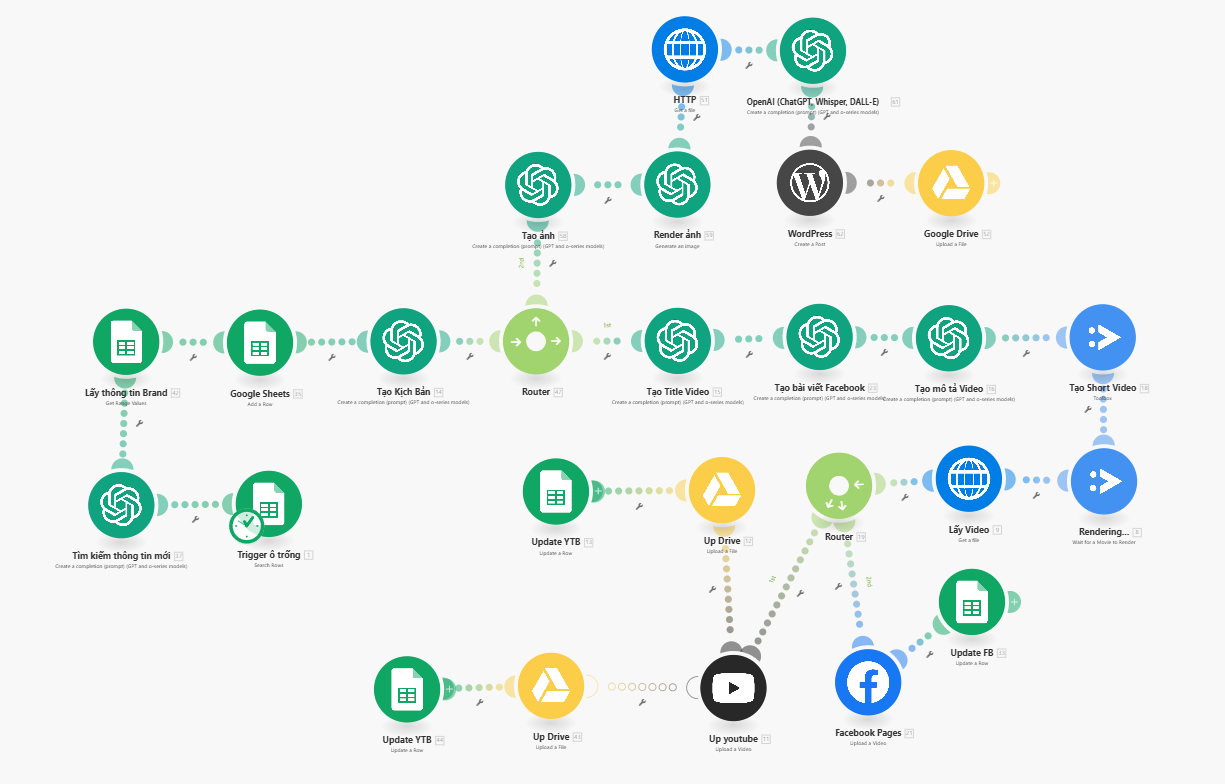
\includegraphics[width=0.6\textwidth]{img/Picture10.png}
    \caption{Workflow truyền thông đa kênh Make.com}
    \label{fig:workflow-make}
\end{figure}

\subsubsection{Workflow tự động tạo nội dung và Video truyền thông đa kênh}

\begin{figure}[h!]
    \centering
    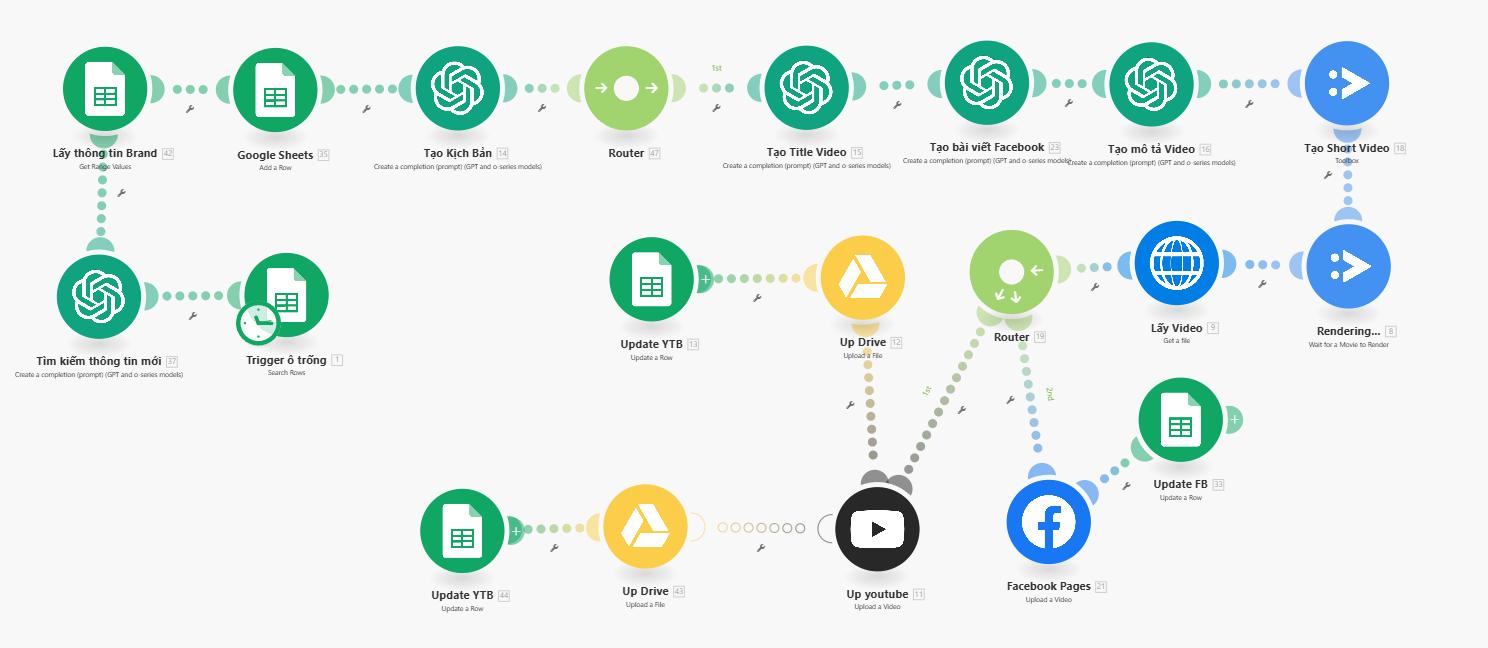
\includegraphics[width=0.6\textwidth]{img/Picture11.png}
    \caption{Workflow tự động tạo nội dung và Video truyền thông đa kênh}
    \label{fig:workflow-video}
\end{figure}

\subsubsection{Workflow tự động tạo bài viết và hình truyền thông Wordpress}

\begin{figure}[h!]
    \centering
    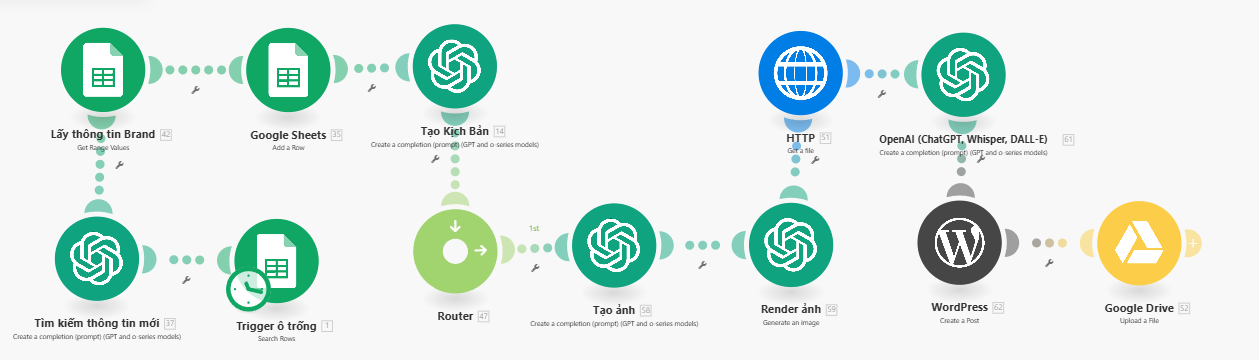
\includegraphics[width=0.6\textwidth]{img/Picture12.png}
    \caption{Workflow tự động tạo bài viết và hình truyền thông Wordpress}
    \label{fig:workflow-wordpress}
\end{figure}

\subsubsection{Kết quả Workflow tự động truyền thông đa kênh}

\begin{figure}[H]
    \centering
    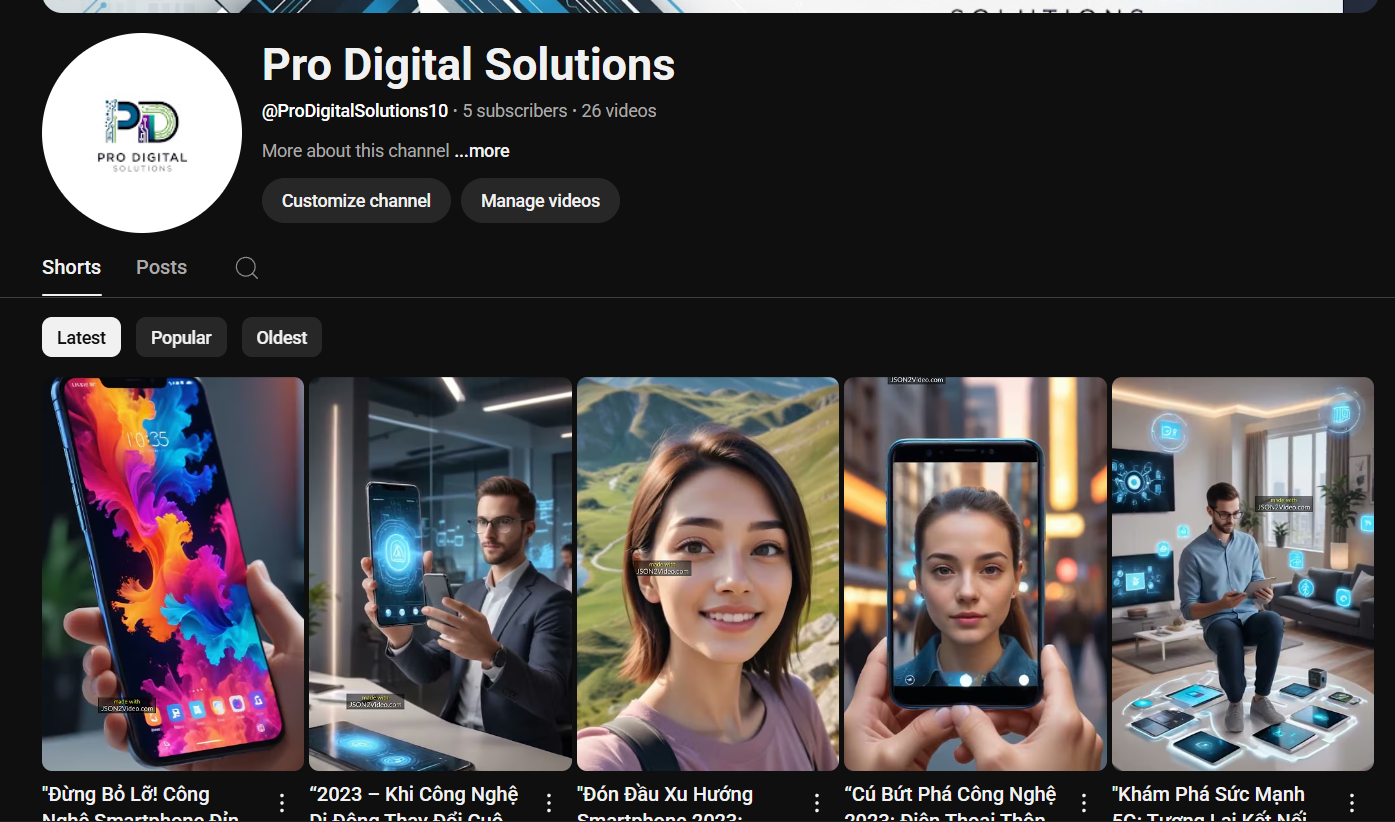
\includegraphics[width=0.6\textwidth]{img/Picture13.png}
    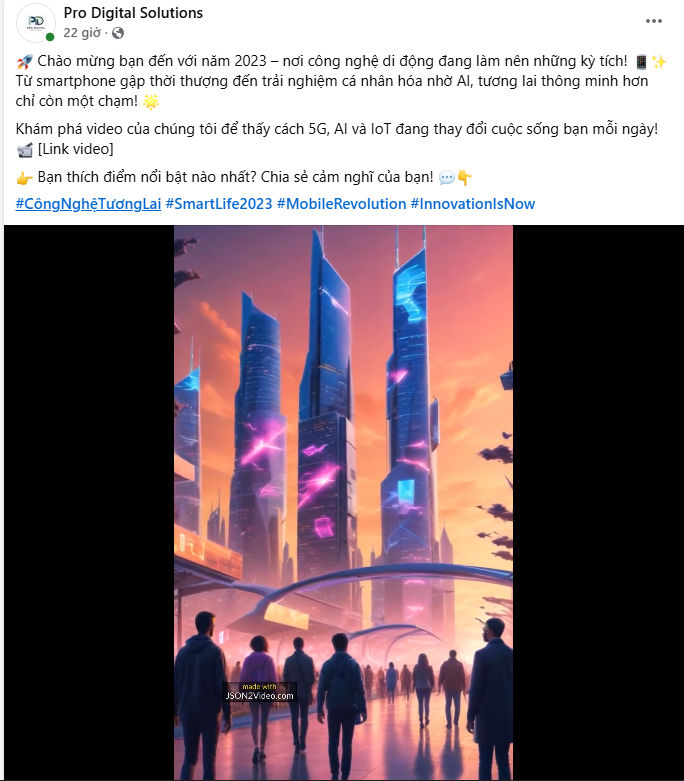
\includegraphics[width=0.6\textwidth]{img/Picture14.png}
    \caption{Kết quả Workflow tự động truyền thông đa kênh}
    \label{fig:workflow-ketqua}
\end{figure}

\subsubsection{Workflow Chatbot Zalo phân loại và trả lời tin nhắn}

\begin{figure}[H]
    \centering
    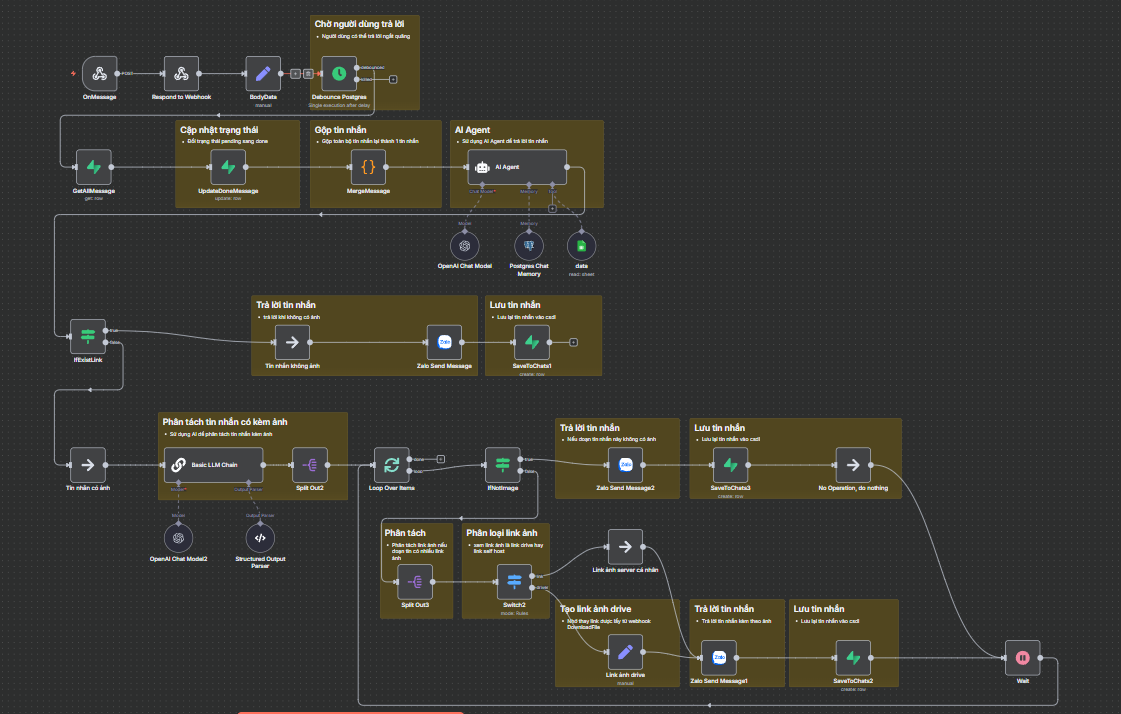
\includegraphics[width=0.6\textwidth]{img/Picture15.png}
    \caption{Workflow chatbot Zalo phân loại và trả lời tin nhắn}
    \label{fig:chatbot-phanloai}
\end{figure}

\subsubsection{Workflow chatbot Zalo tiếp nhận tin nhắn, phân loại và lưu trữ}

\begin{figure}[H]
    \centering
    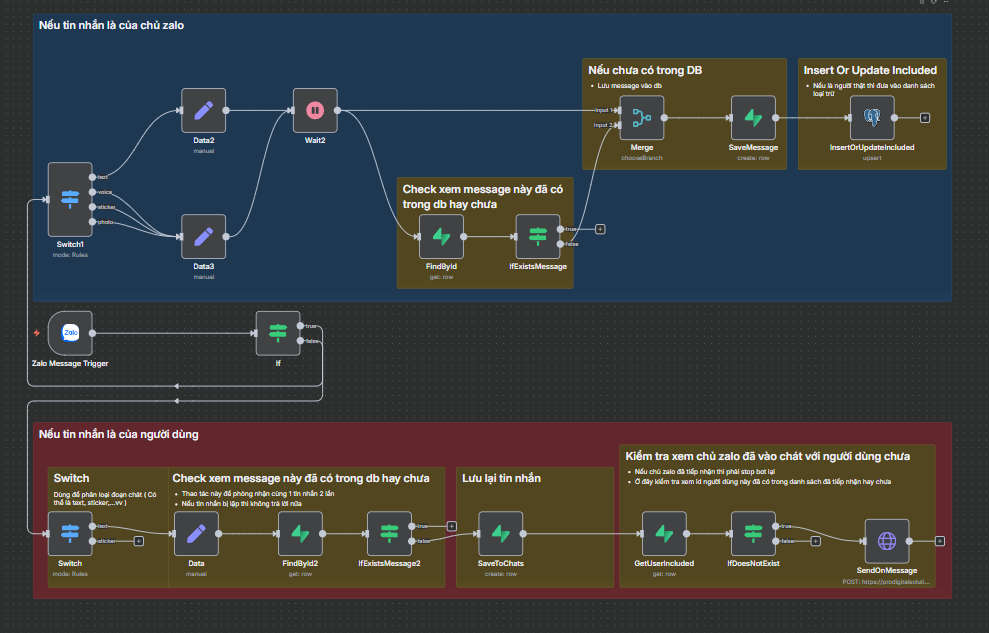
\includegraphics[width=0.6\textwidth]{img/Picture16.png}
    \caption{Workflow chatbot Zalo tiếp nhận tin nhắn, phân loại và lưu trữ}
    \label{fig:chatbot-luutru}
\end{figure}

\subsubsection{Workflow tải hình ảnh từ Google Drive và khởi tạo cơ sở dữ liệu}

\begin{figure}[H]
    \centering
    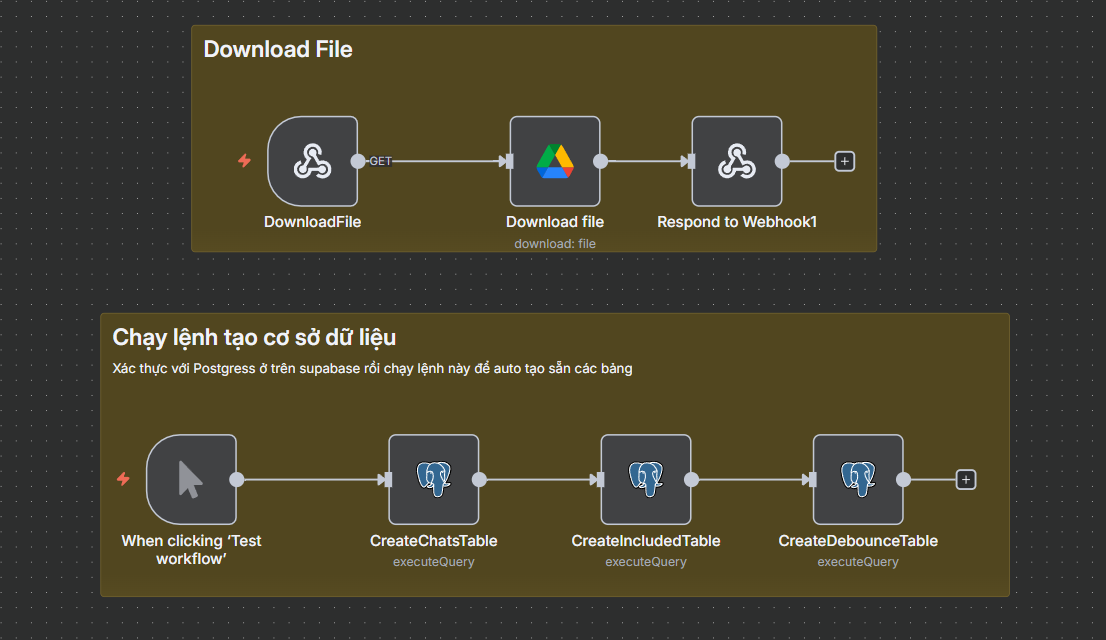
\includegraphics[width=0.6\textwidth]{img/Picture17.png}
    \caption{Workflow tải hình ảnh từ Google Drive và khởi tạo cơ sở dữ liệu}
    \label{fig:chatbot-drive}
\end{figure}



\subsubsection{Kết quả Chatbot Zalo hỗ trợ tư vấn khách hàng}
\begin{figure}[H]
    \centering
    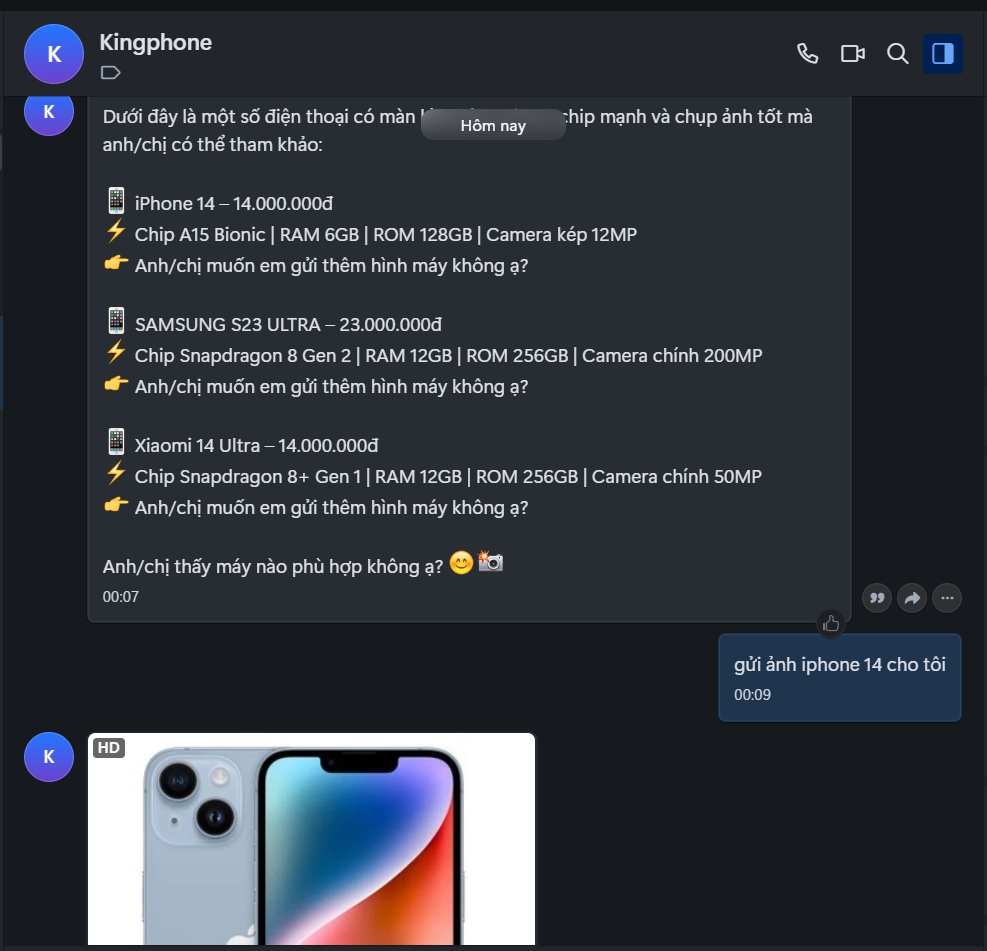
\includegraphics[width=0.6\textwidth]{img/Picture18.png}
    \caption{Kết quả Chatbot Zalo hỗ trợ tư vấn khách hàng}
    \label{fig:chatbot-ketqua1}
    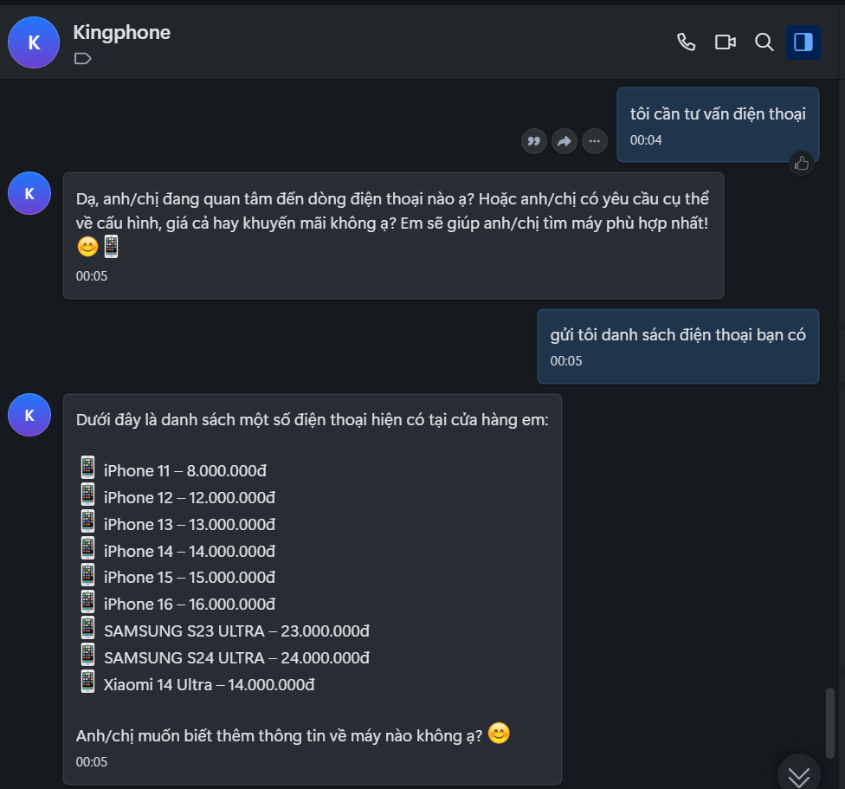
\includegraphics[width=0.6\textwidth]{img/Picture19.png}
    \caption{Kết quả Chatbot Zalo hỗ trợ tư vấn khách hàng}
    \label{fig:chatbot-ketqua}
\end{figure}
\subsection{Wordpress}

\subsubsection{Trang chủ}
\begin{figure}[H]
    \centering
    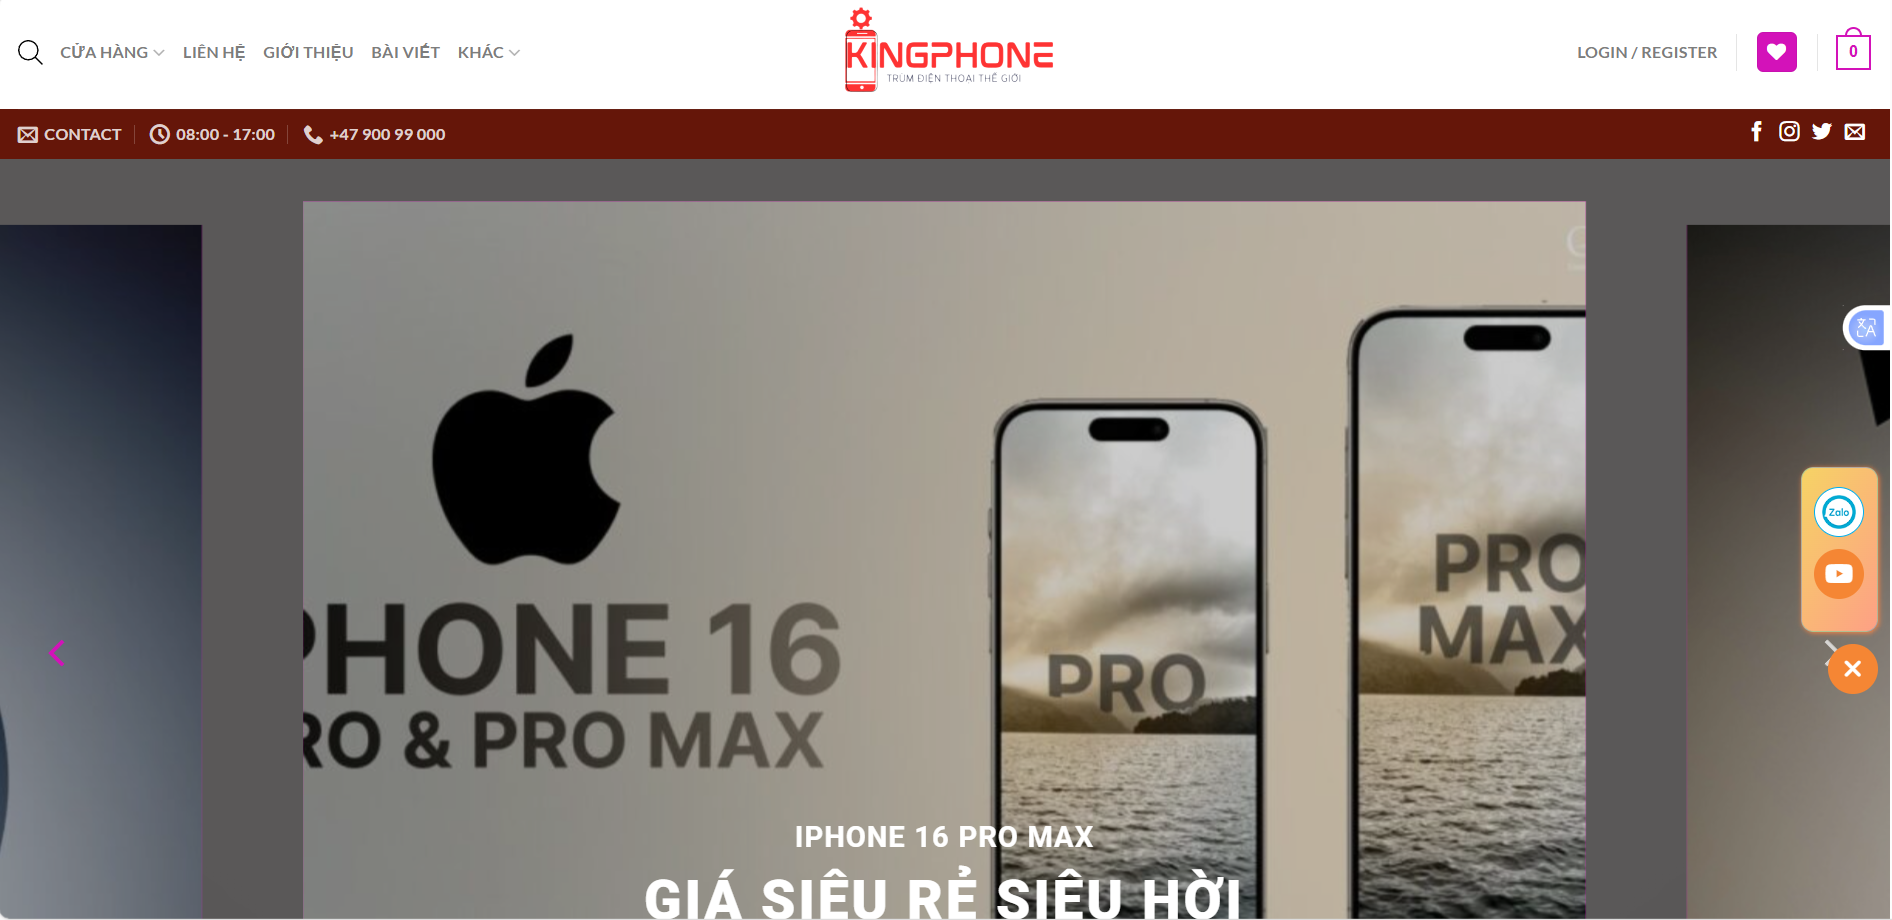
\includegraphics[width=0.6\textwidth]{img/trangchu1.png}
    \caption{Trang chủ 1}
    \label{fig:tc}
\end{figure}
\subsubsection{Header}
\begin{figure}[H]
    \centering
    
\includegraphics[width=0.6\textwidth]{img/header.png}
    \caption{Trang Header}
    \label{fig:header}
\end{figure}
\subsubsection{Footer}
\begin{figure}[H]
    \centering
    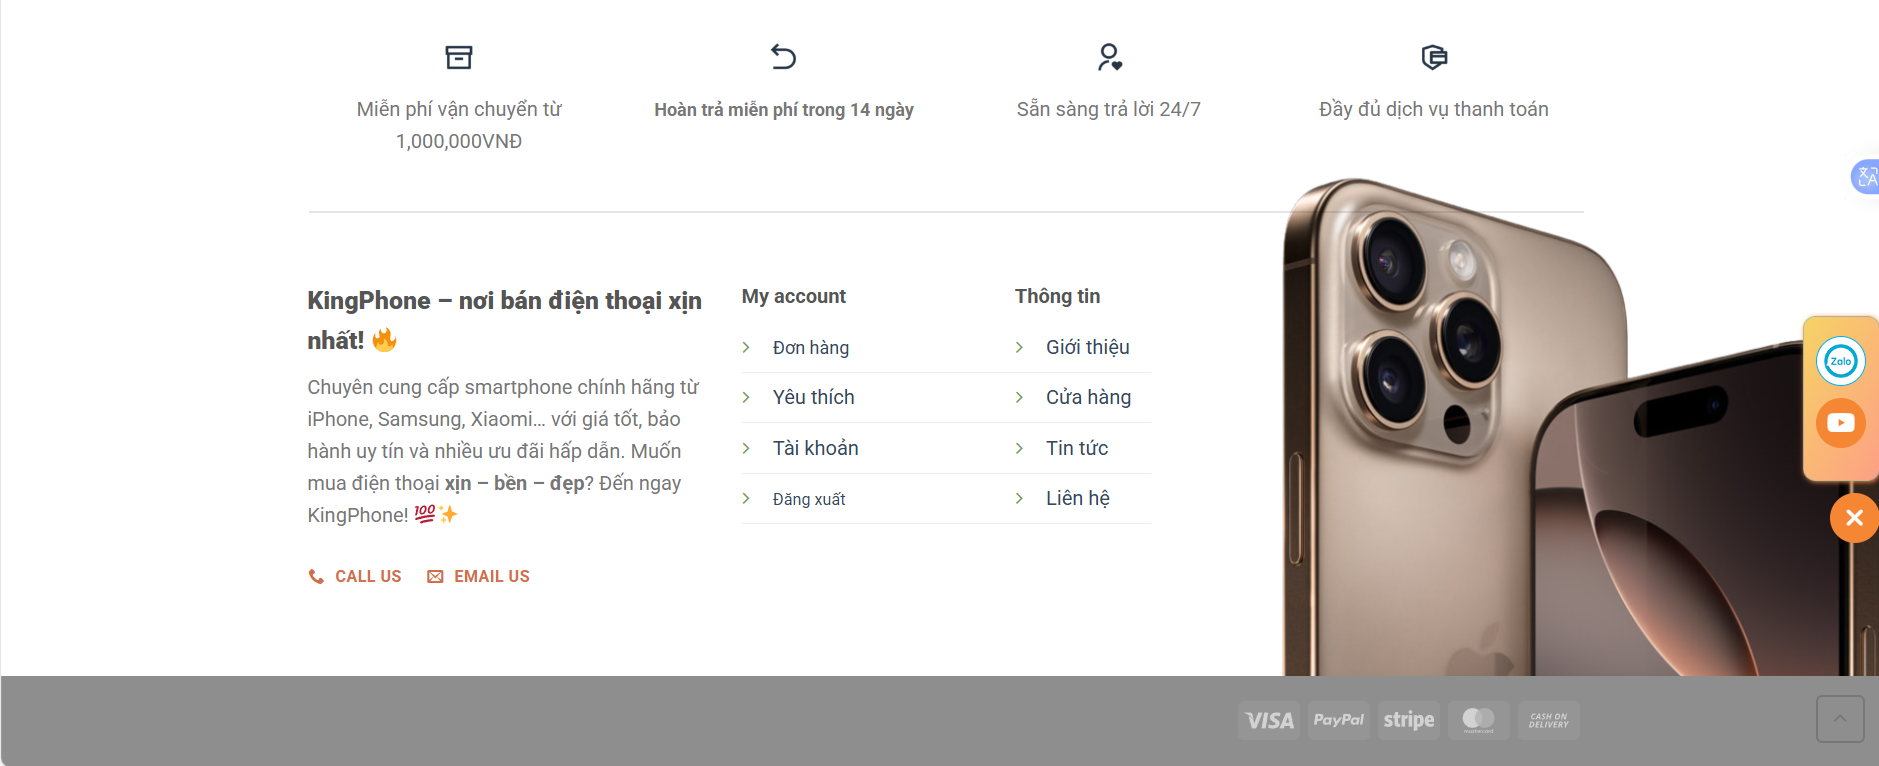
\includegraphics[width=0.6\textwidth]{img/footer.png}
    \caption{Trang Footer}
    \label{fig:foter}
\end{figure}
\subsubsection{Trang Đăng ký/ Đăng nhập}
\begin{figure}[H]
    \centering
    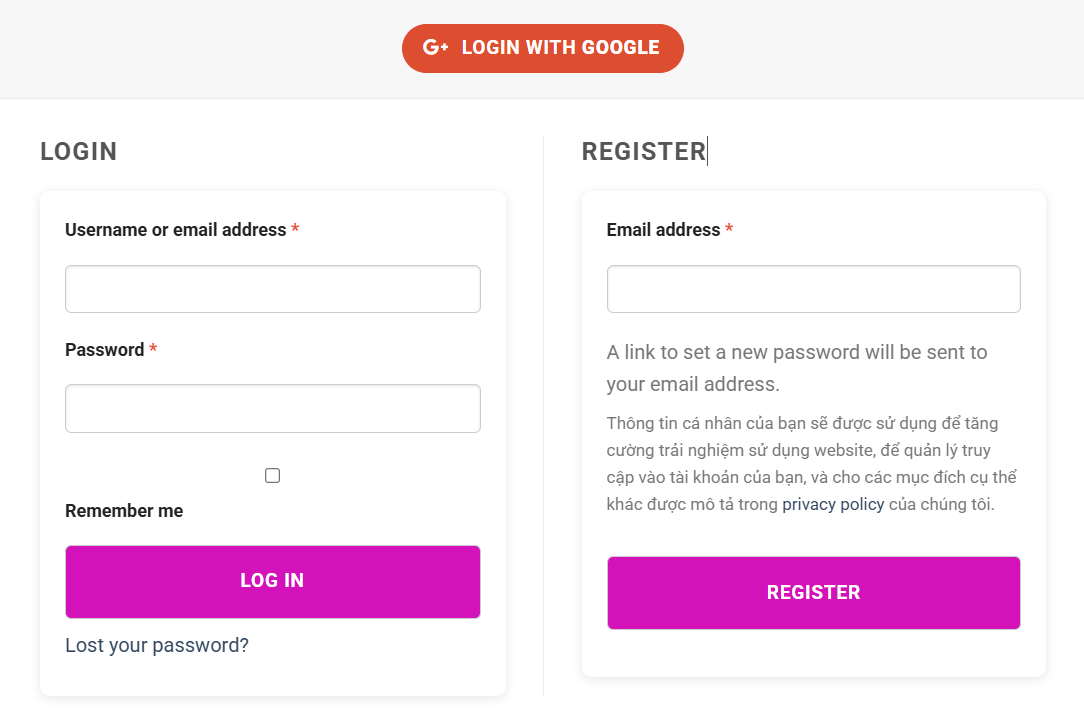
\includegraphics[width=0.6\textwidth]{img/dangnhap.png}
    \caption{Trang đăng ký/đăng nhập}
    \label{fig:dkdn}
\end{figure}

\subsubsection{Trang sản phẩm}
\begin{figure}[H]
    \centering
    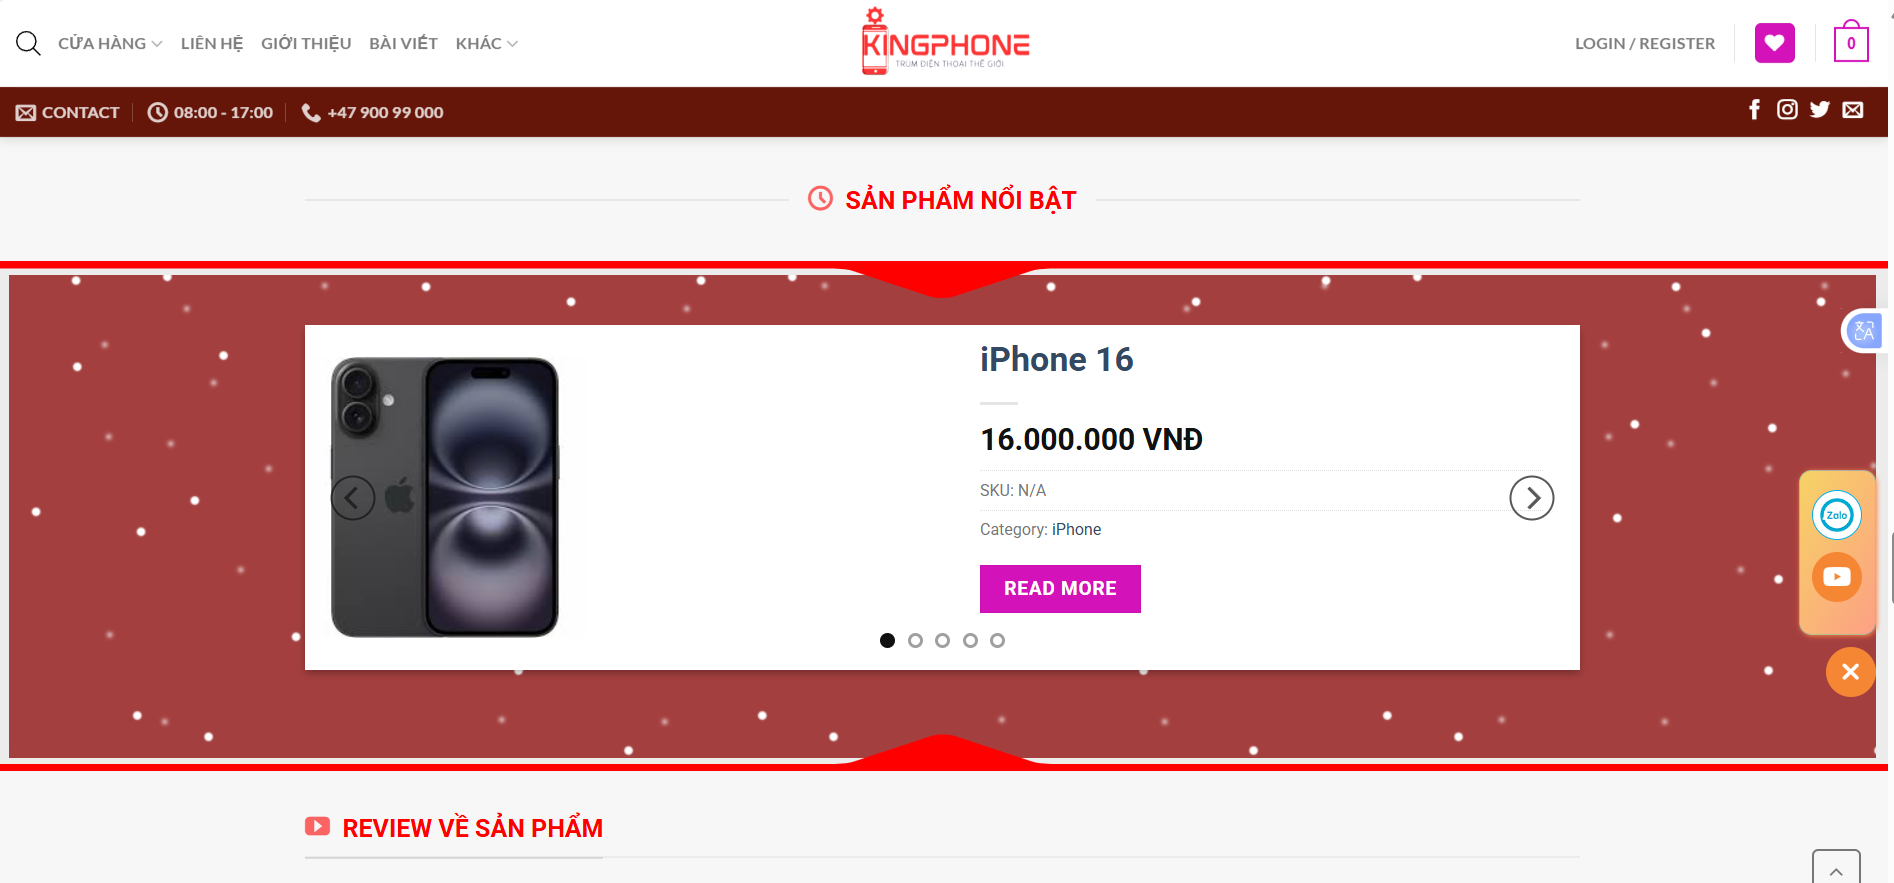
\includegraphics[width=0.6\textwidth]{img/sanpahmnoibat.png}
    \caption{Trang sản phẩm nổi bật}
    \label{fig:noibat}
\end{figure}

\subsubsection{Trang sản phẩm}
\begin{figure}[H]
    \centering
    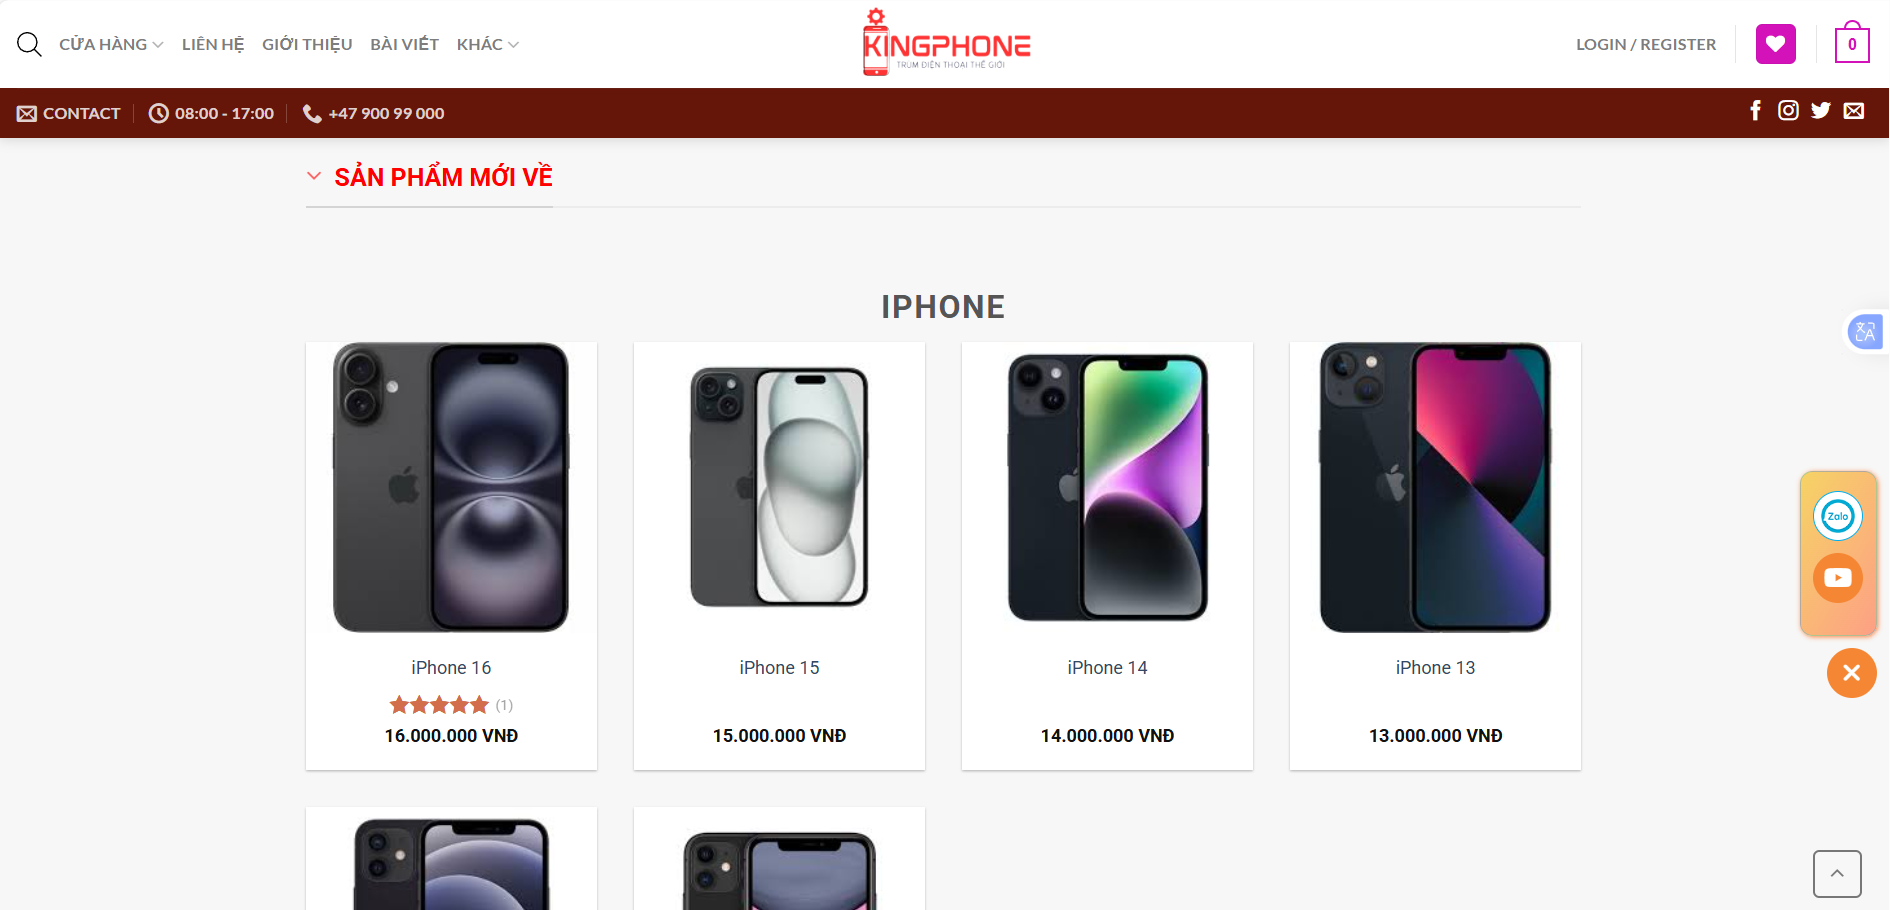
\includegraphics[width=0.6\textwidth]{img/sanphammoive.png}
    \caption{Trang sản phẩm mới về}
    \label{fig:moive}
\end{figure}


\subsubsection{Trang Reviews sản phẩm}
\begin{figure}[H]
    \centering
    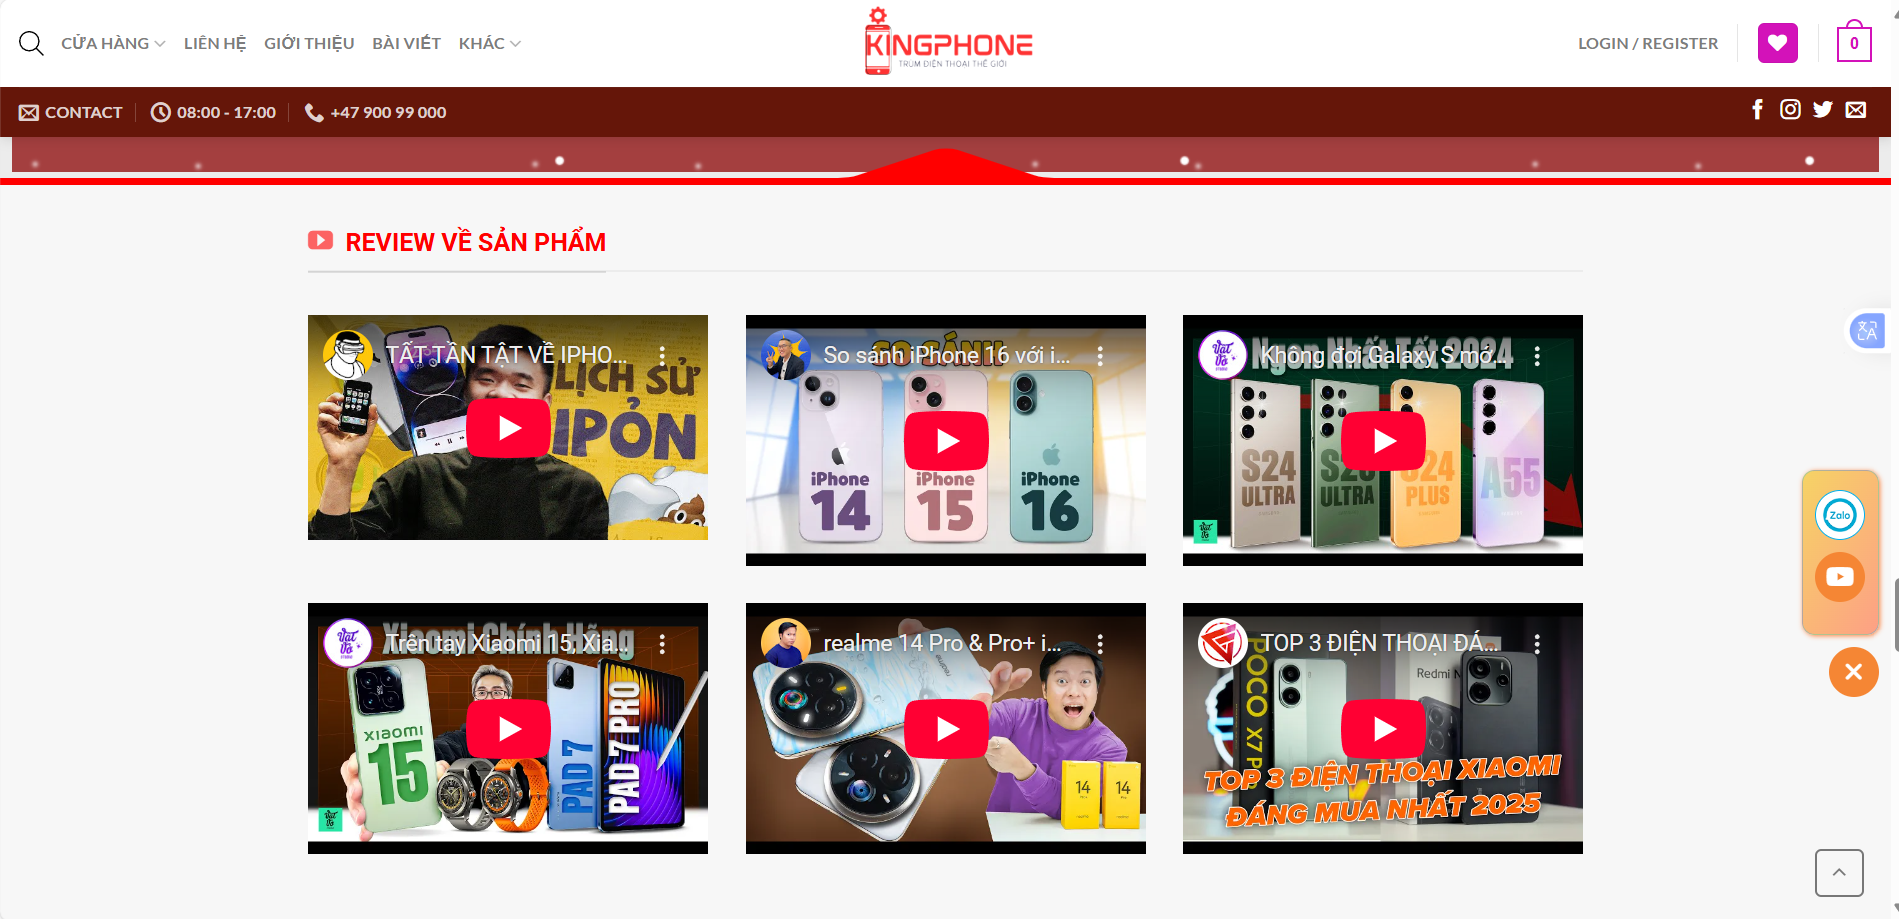
\includegraphics[width=0.6\textwidth]{img/reviewsp.png}
    \caption{Trang Reviews sản phẩm }
    \label{fig:rv}
\end{figure}

\subsubsection{Trang sản phẩm yêu thích}
\begin{figure}[H]
    \centering
    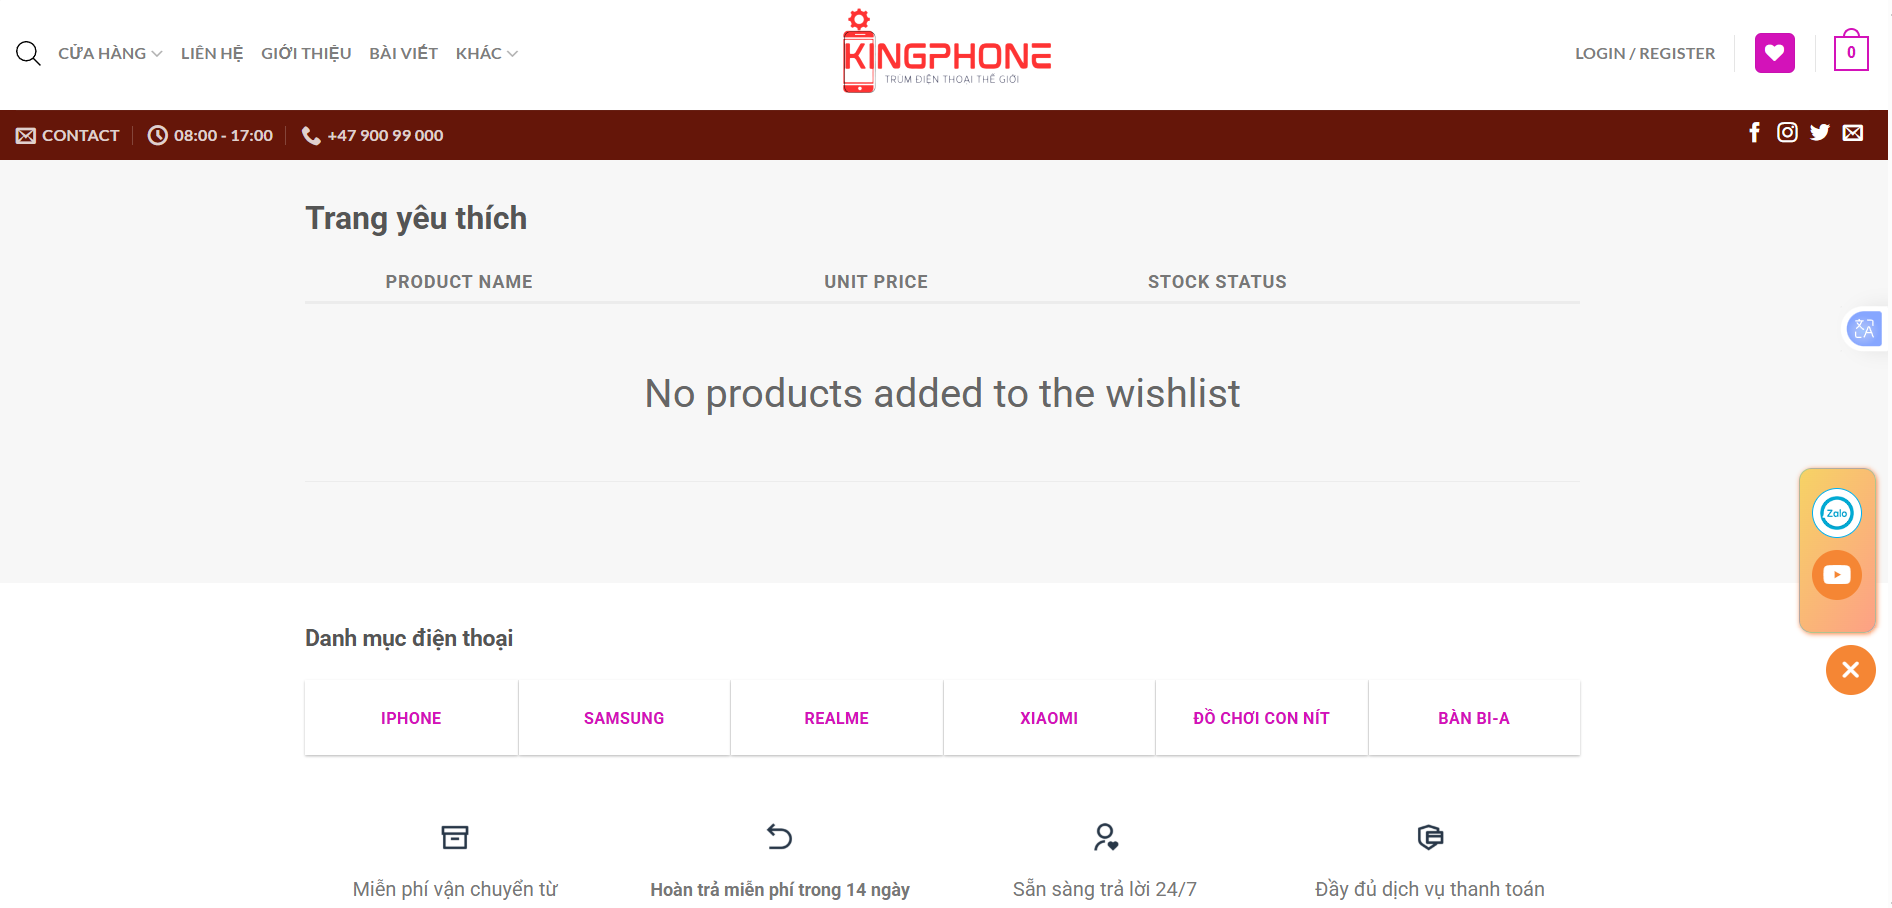
\includegraphics[width=0.6\textwidth]{img/sanphamyeuthich.png}
    \caption{Trang sản phẩm yêu thích}
    \label{fig:yeu}
\end{figure}

\subsubsection{Trang giỏ hàng}
\begin{figure}[H]
    \centering
    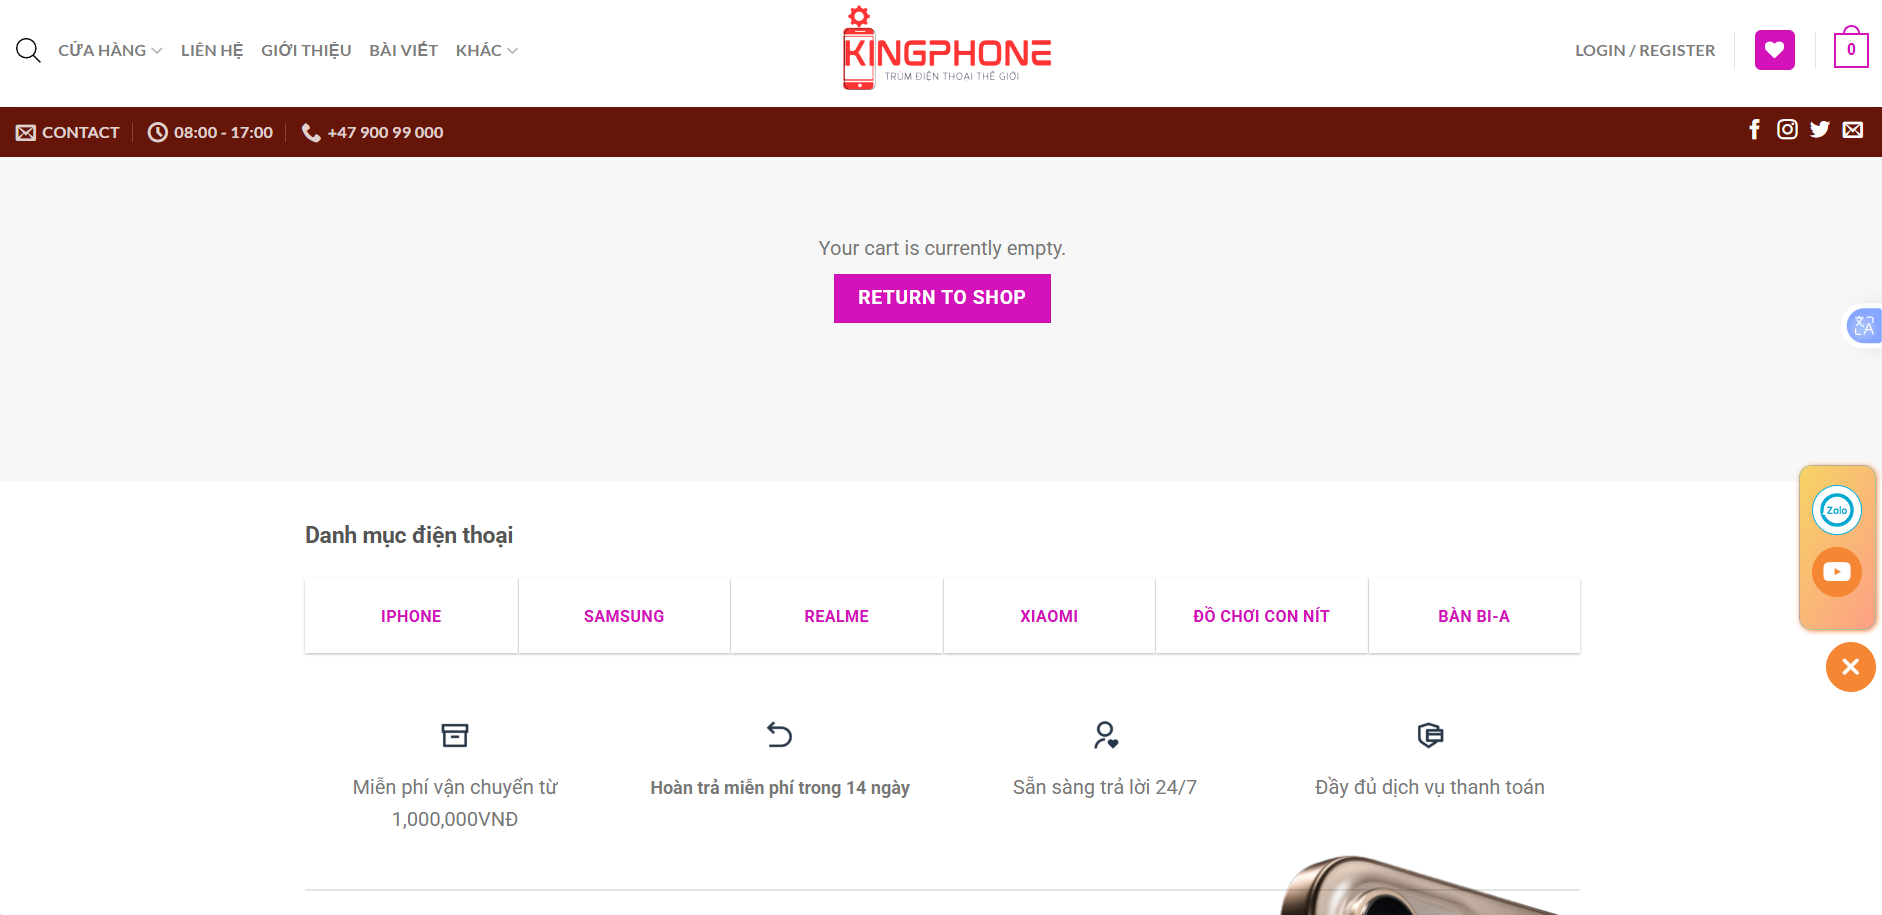
\includegraphics[width=0.6\textwidth]{img/giohang.png}
    \caption{Trang giỏ hàng}
    \label{fig:giohang}
\end{figure}

\subsubsection{Trang liên hệ}
\begin{figure}[H]
    \centering
    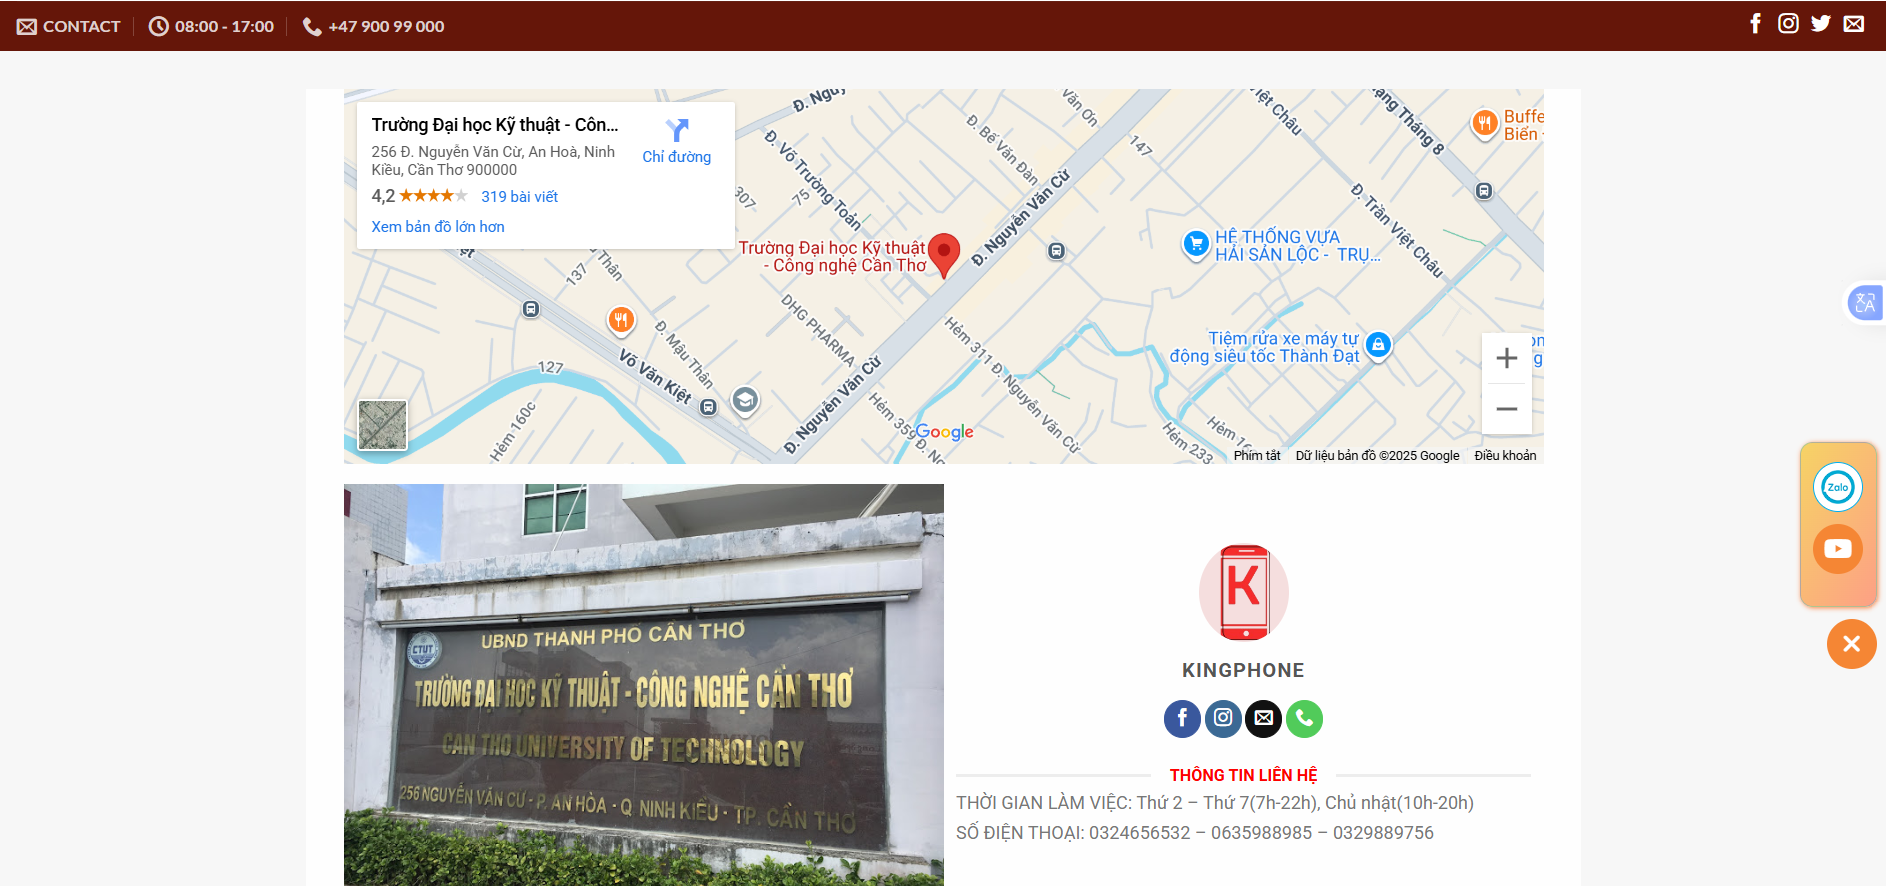
\includegraphics[width=0.6\textwidth]{img/lienhe.png}
    \caption{Trang liên hệ}
    \label{fig:lh}
\end{figure}

\subsubsection{Trang liên hệ}
\begin{figure}[H]
    \centering
    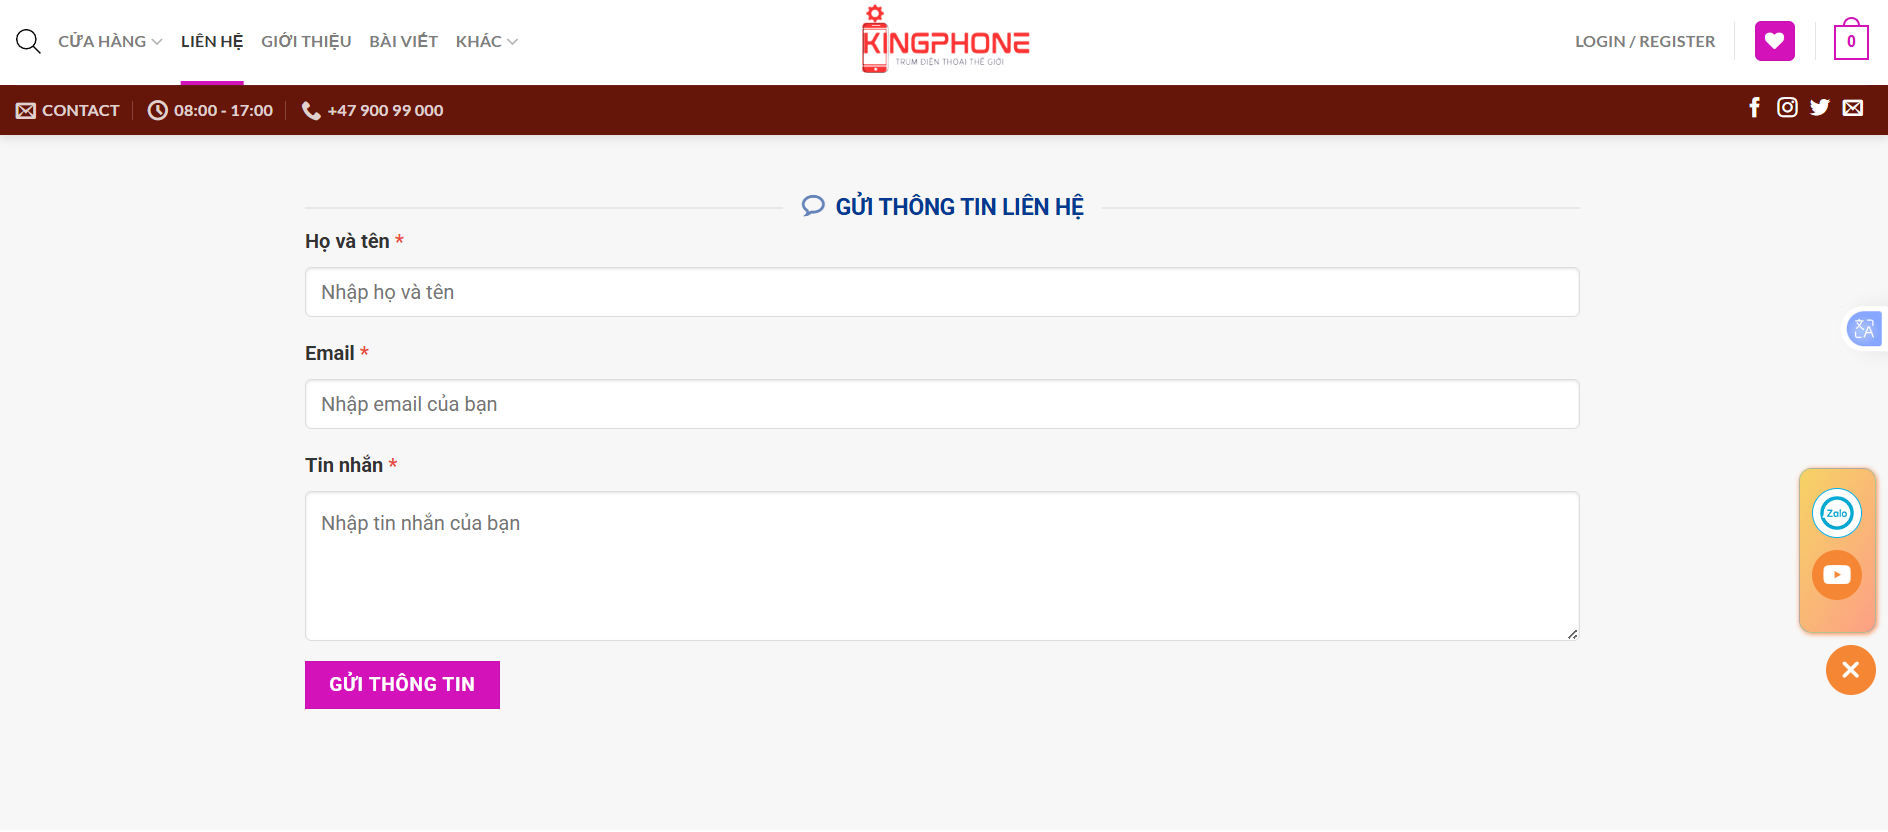
\includegraphics[width=0.6\textwidth]{img/guithongtinlienhe.png}
    \caption{Trang gửi thông tin liên hệ}
    \label{fig:noibat}
\end{figure}

\subsubsection{Trang giới thiệu}
\begin{figure}[H]
    \centering
    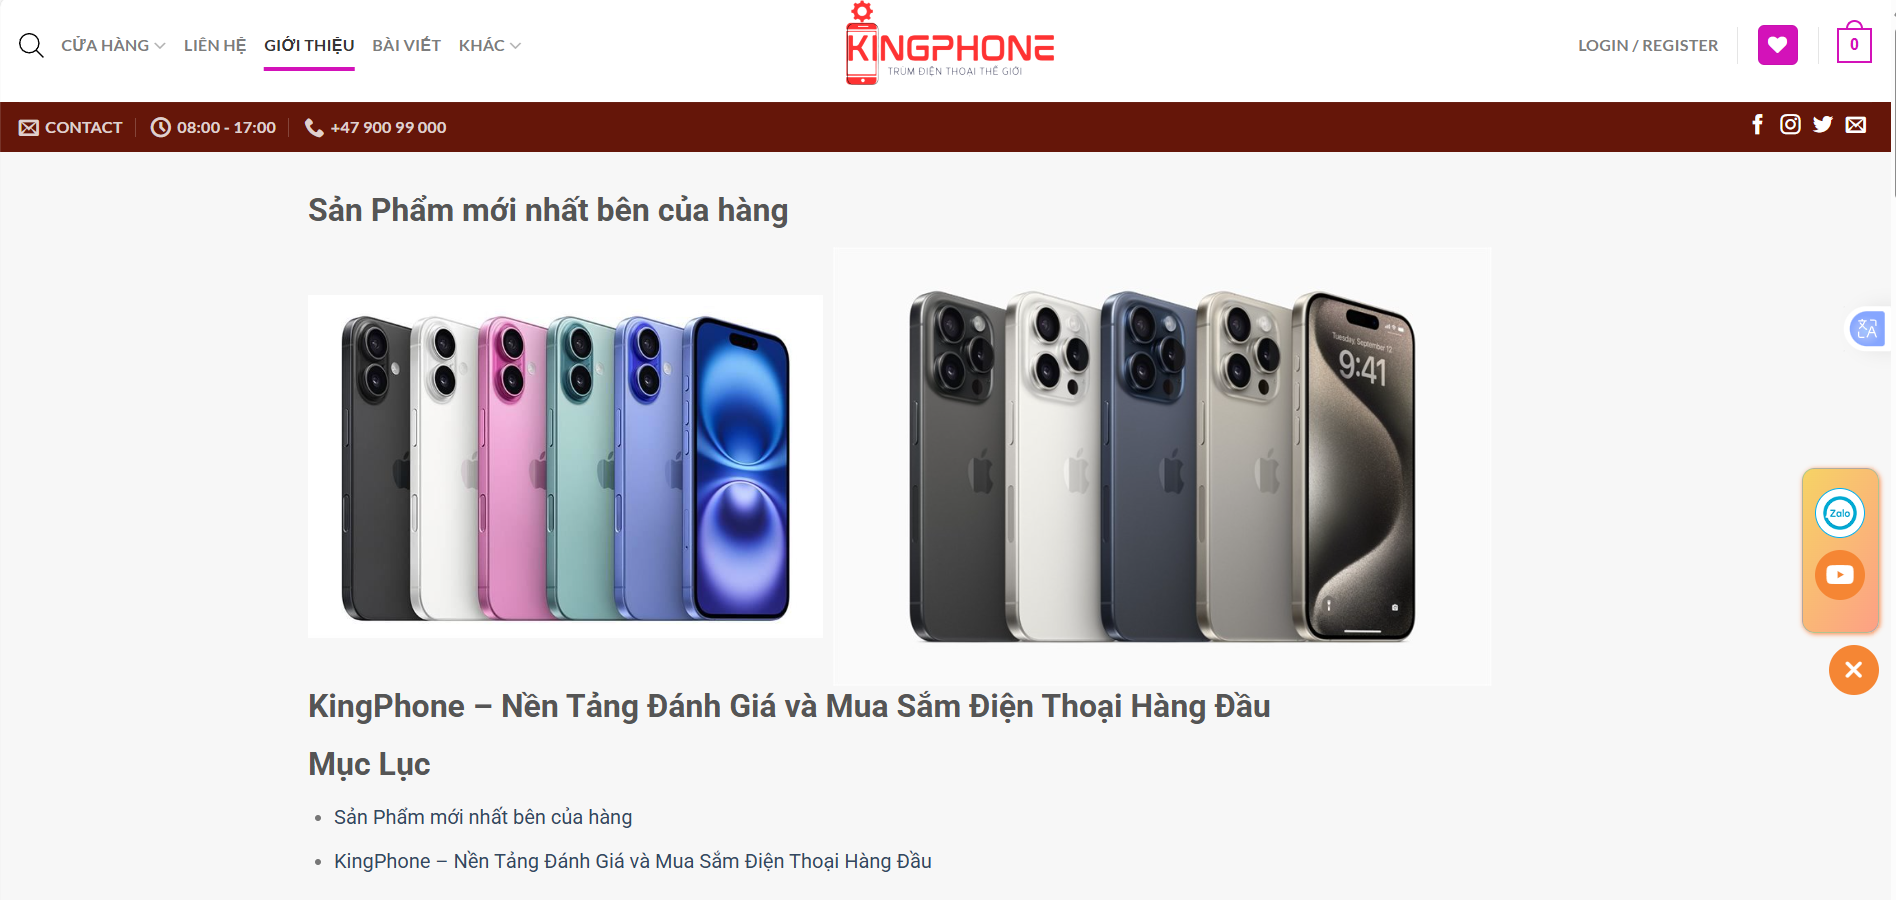
\includegraphics[width=0.6\textwidth]{img/gioithieu.png}
    \caption{Trang giới thiệu}
    \label{fig:gt}
\end{figure}

\subsubsection{Trang bài viết}
\begin{figure}[H]
    \centering
    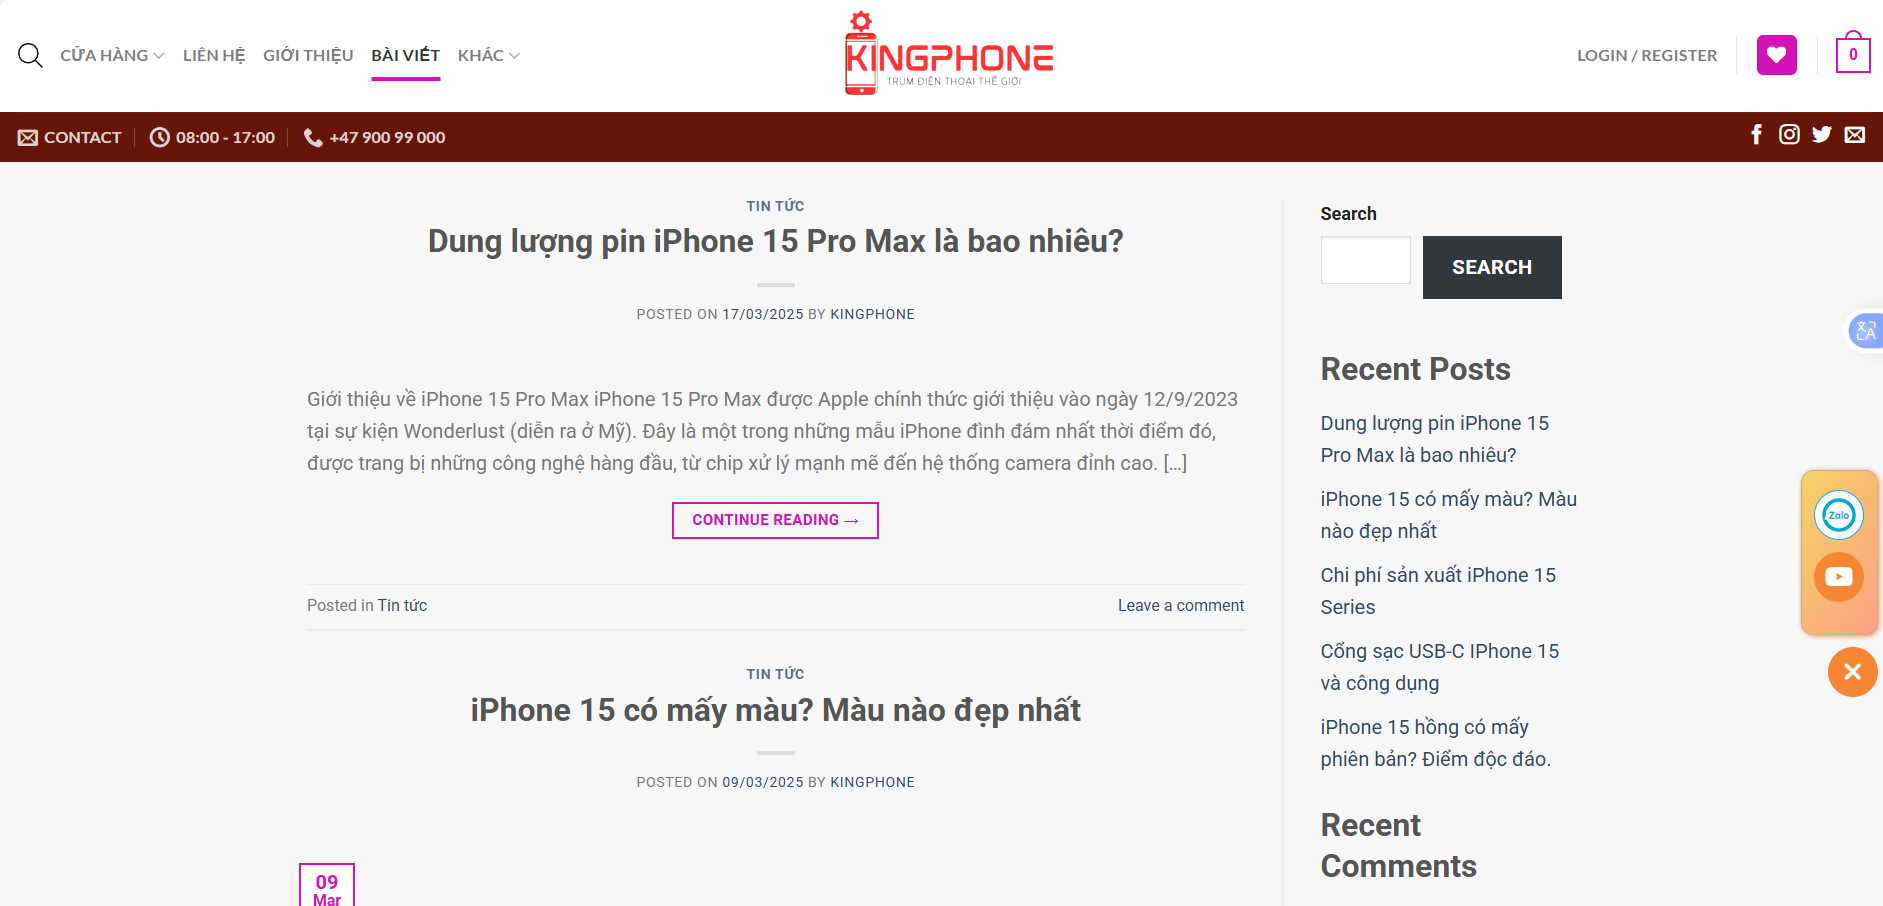
\includegraphics[width=0.6\textwidth]{img/baiviet.png}
    \caption{Trang bài viết}
    \label{fig:baiviet}
\end{figure}

\subsubsection{Trang bảo mật}
\begin{figure}[H]
    \centering
    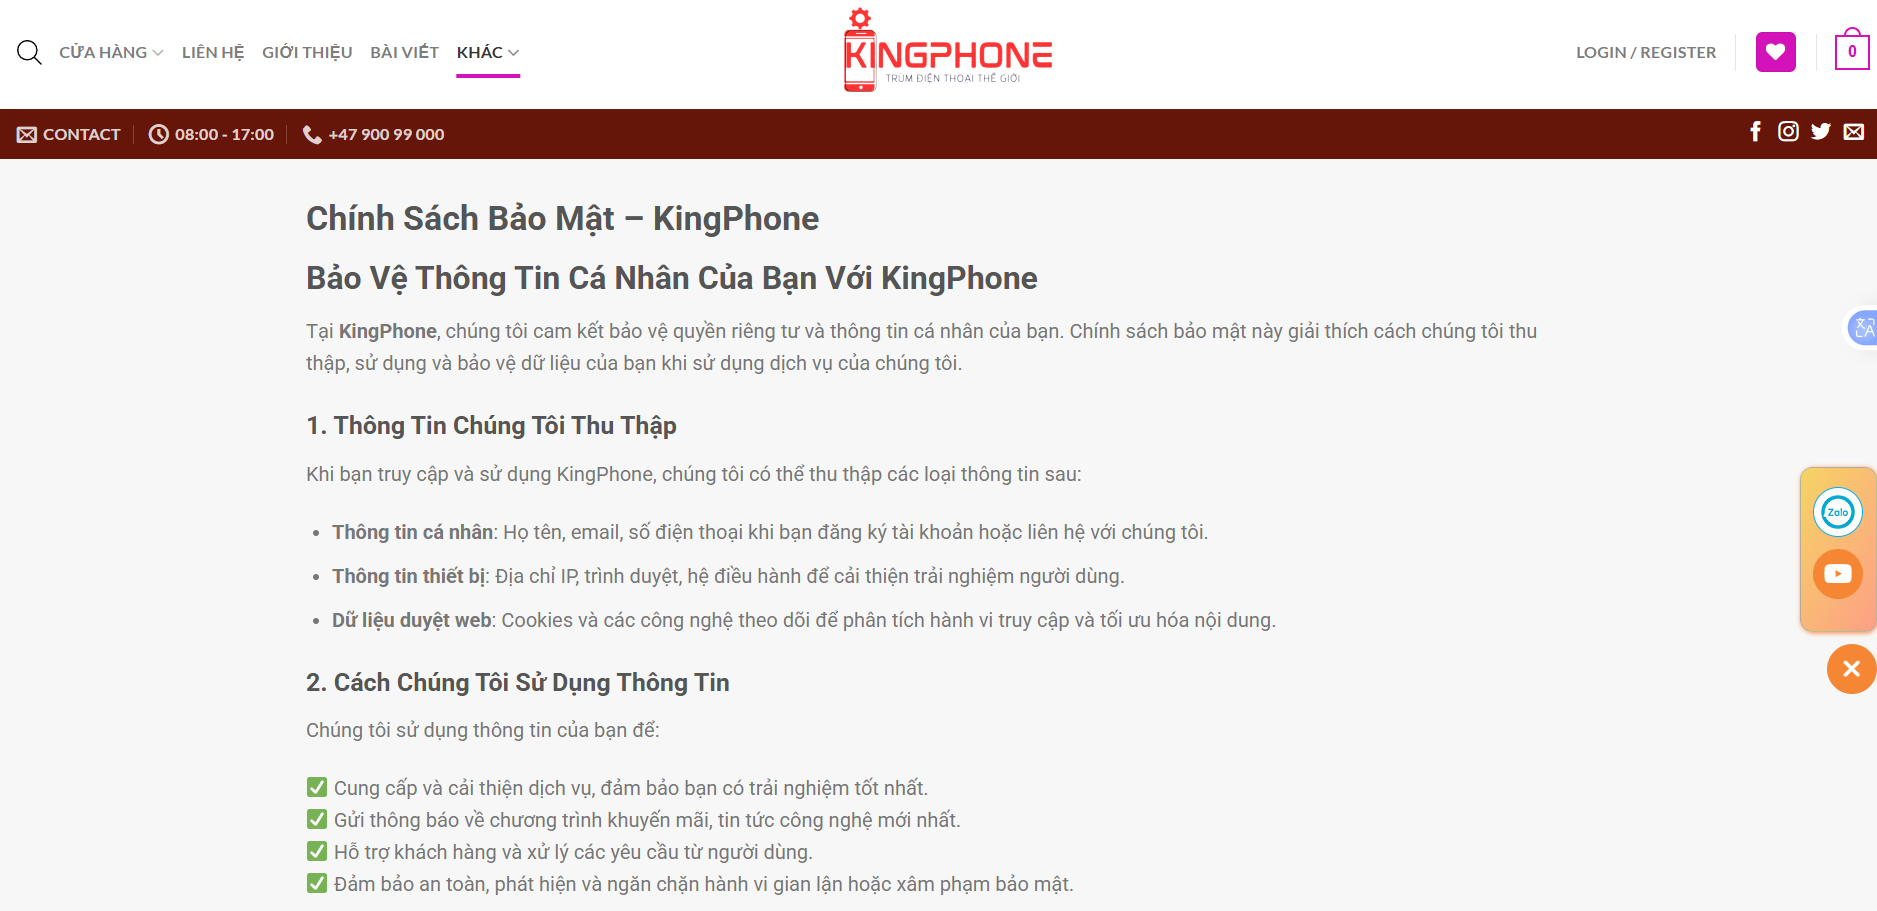
\includegraphics[width=0.6\textwidth]{img/baomat.png}
    \caption{Trang bảo mật}
    \label{fig:bmat}
\end{figure}

\subsubsection{Trang điều khoản}
\begin{figure}[H]
    \centering
    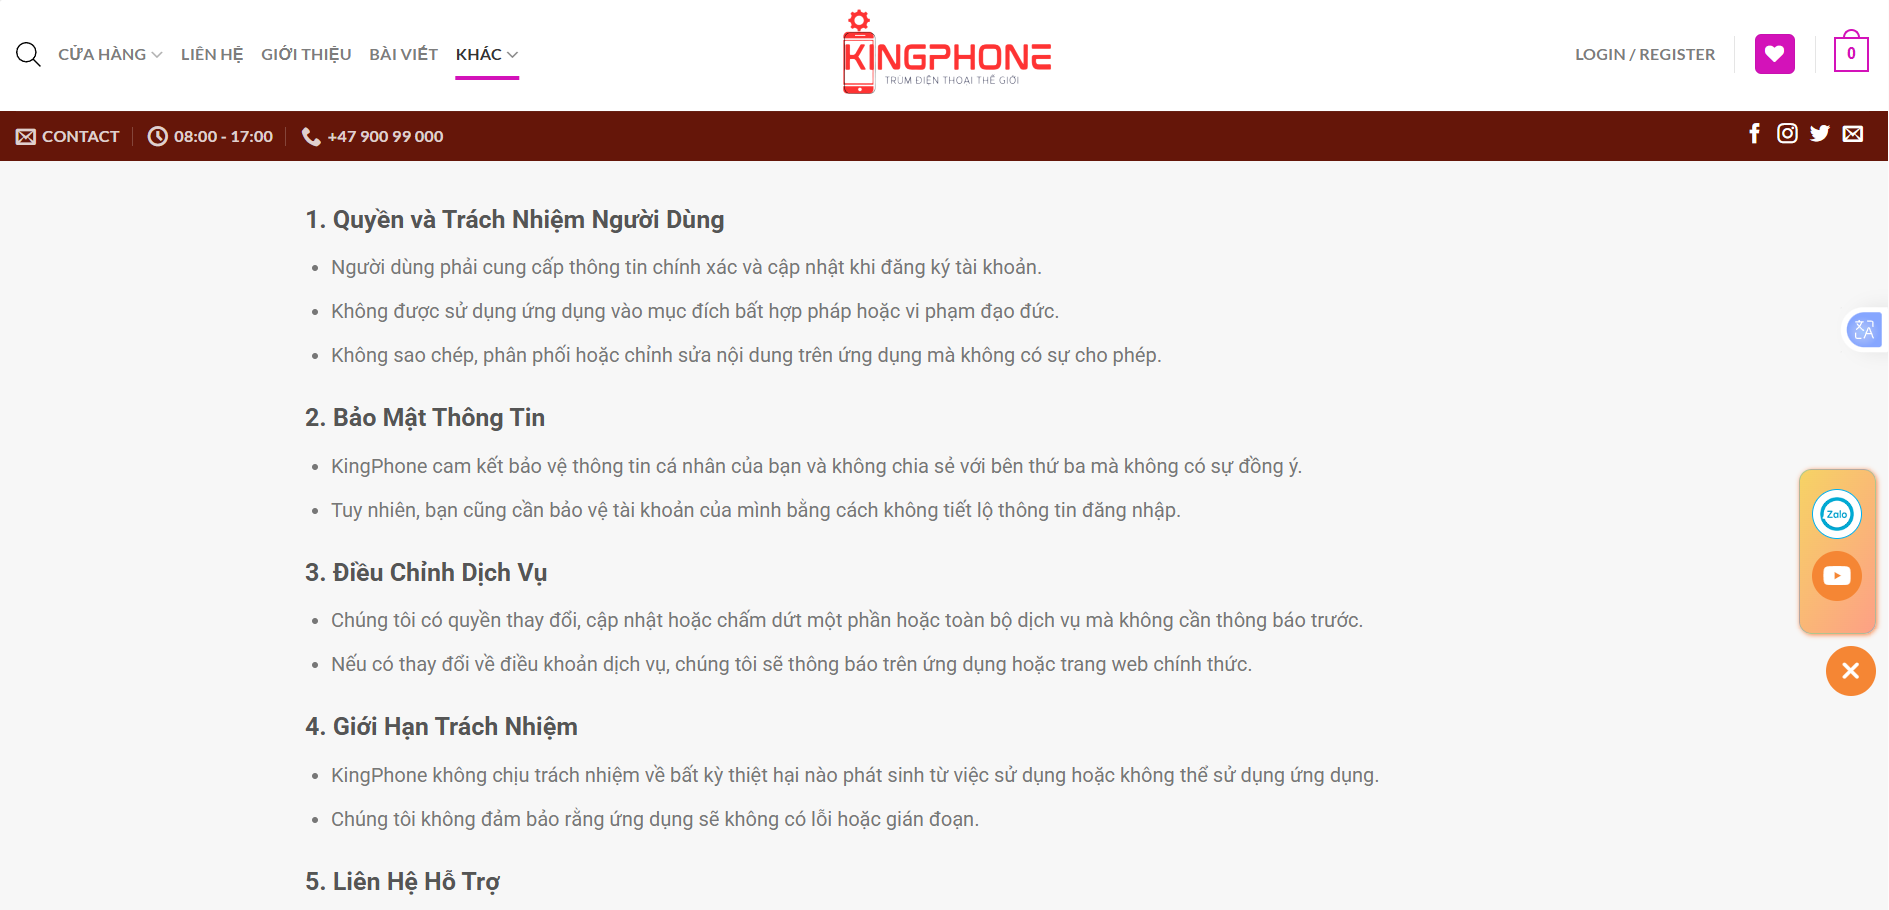
\includegraphics[width=0.6\textwidth]{img/dieukhoan.png}
    \caption{Trang điều khoản}
    \label{fig:dkhoan}
\end{figure}

\subsubsection{Trang tìm kiếm}
\begin{figure}[H]
    \centering
    
\includegraphics[width=0.6\textwidth]{img/timkiem.png}
    \caption{Trang tìm kiếm}
    \label{fig:tkiem}
\end{figure}

\section*{Kết luận chương}
Qua quá trình thực tập và triển khai đề tài, tôi đã hiểu rõ hơn về tầm quan trọng
của việc ứng dụng công nghệ tự động hóa trong hoạt động truyền thông và thương mại
điện tử. Hệ thống Chatbot Zalo đã chứng minh được khả năng hỗ trợ hiệu quả cho
doanh nghiệp, từ tiết kiệm nguồn lực, nâng cao trải nghiệm khách hàng đến hỗ trợ
marketing. Tuy nhiên, để đạt được hiệu quả toàn diện, hệ thống cần được tiếp tục cải
tiến theo các giải pháp đã đề xuất. Đây cũng chính là hướng phát triển trong tương lai,
góp phần giúp doanh nghiệp bắt kịp xu hướng chuyển đổi số.
